\documentclass[fleqn,10pt]{olplainarticle}
% Use option lineno for line numbers 

\title{Pan-Cancer Multi-Agent Tumor Segmentation and Analysis with Conditional Probabilistic Anatomical Reasoning}

\author[1]{First Author}
\author[2]{Second Author}
\affil[1]{Address of first author}
\affil[2]{Address of second author}

\keywords{Keyword1, Keyword2, Keyword3}

\begin{abstract}
Please provide an abstract of no more than 300 words. Your abstract should explain the main contributions of your article, and should not contain any material that is not included in the main text. 
\end{abstract}

\begin{document}

\flushbottom
\maketitle
\thispagestyle{empty}

\section{Introduction}

\begin{itemize}
    \item Build a pan-cancer multi-agent tumor segmentation system
    \item 2D, 3D tumor segmentation models, anatomical segmentation models could be any, even allow users to define or use their private models
    \item Beyond segmentation, provide anatomical graph and explanation
\end{itemize}

\section{Methodology}
\label{sec:method}
% Condensed 26 Oct 2026 (Claude, with the user): the main text keeps the model and its key equations; implementation details,
% rules and constants moved to Appendices A--D; repeated statements removed; stage-2 text updated to the implementation
% (within-scan appearance priors, background mixing weights, multi-lesion simulation, matched-flexibility Bayes factor).
% Backup of the previous version: clinical/PanCIA_outputs/paper_outputs/main_tex_backups/main_before_method_condense_20261026.tex.
\begin{figure*}[t]
    \centering
    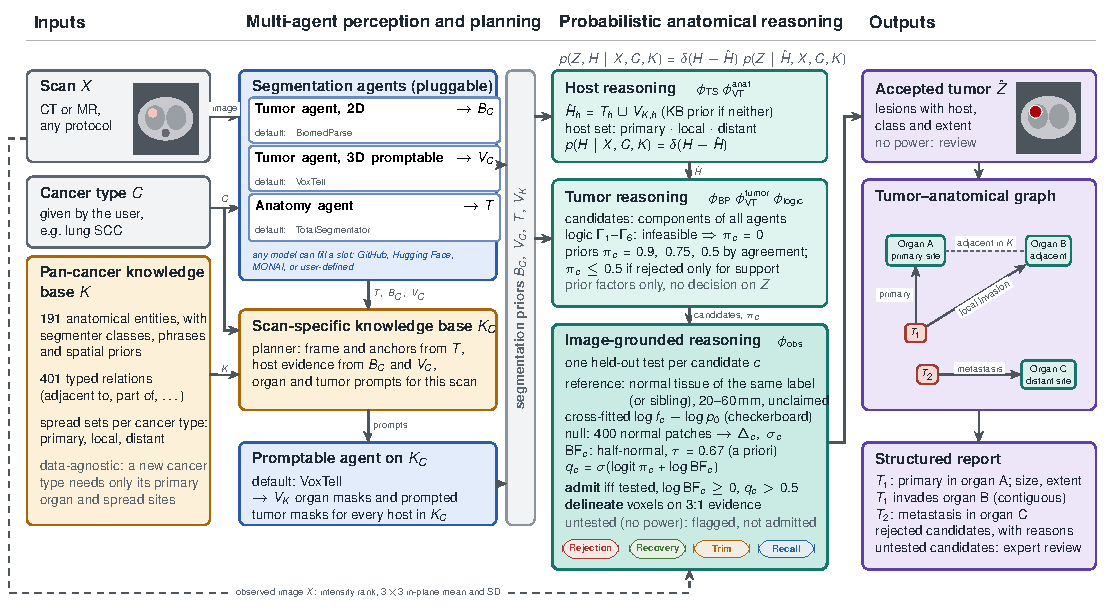
\includegraphics[width=\linewidth]{figs/pipeline.pdf}
    \caption{Pan-cancer multi-agent tumor segmentation and reasoning. Given a scan $X$ and a user-given cancer type $C$,
    pluggable segmentation agents produce tumor and anatomy masks, guided by a scan-specific prompt plan $K_C$ derived from
    the pan-cancer knowledge base $K$. Stage~1 localizes tumors: set-based reasoning turns the masks into anchors with host
    candidates, support levels and candidate extents; the host is inferred from anatomy as a credible set, existence is tested
    against expert likelihoods, and an extent is chosen among the agents' outlines. Stage~2 segments each localized tumor
    voxel by voxel with a Bayesian model whose priors come from stage~1 and from expert annotations.
    [figure to be updated for stage 2]}
    \label{fig:pipeline}
\end{figure*}

Given a scan $X$ and its cancer type $C$, the framework runs in two stages (Fig.~\ref{fig:pipeline}). Pluggable
segmentation agents propose tumors and anatomy (Section~\ref{sec:agents}). Stage~1 \emph{localizes} the tumors: it
reasons over the agents' masks and an anatomical knowledge base to decide, for each candidate, whether it is a tumor,
which organ hosts it and which of the agents' outlines delineates it (Section~\ref{sec:conditional_reasoning}). Stage~2
\emph{segments} each localized tumor voxel by voxel (Section~\ref{sec:stage2}). Three principles hold throughout.
(i)~Every likelihood, prior and threshold is estimated on public expert annotations, never on agent outputs or on the
evaluated cohort. (ii)~No rule names a cancer type, an agent or a dataset, and patient sex is never used. (iii)~Early steps
generate candidates and decide only what is impossible; competing explanations stay open until the image has been
consulted. Rules, constants and their sources are given in the appendices.

\subsection{Segmentation agents and knowledge base}
\label{sec:agents}
Agents are pluggable and treated equally. A \emph{tumor agent} returns tumor masks for text prompts (a cancer-specific
prompt such as \emph{kidney tumor}, and, if promptable, one prompt per expected host in view); an \emph{organ agent} returns
labelled organ masks. With the default agents (Table~\ref{tab:agents}),
\begin{equation}
\label{eq:agents}
\begin{aligned}
B_C&=f_{\mathrm{BP}}(X,C), & V_C&=f_{\mathrm{VT}}(X,C,K_C),\\
V_K&=f_{\mathrm{VT}}(X,K_C), & T&=f_{\mathrm{TS}}(X),
\end{aligned}
\end{equation}
where $B_C$ and $V_C$ are tumor masks and $V_K$ and $T$ organ masks; $A_{k,o}$ denotes agent $k$'s mask of organ $o$.
Agreement counts agents, not prompts, and every piece of support keeps its provenance, so an agent never confirms its own
proposal.

\begin{table*}[t]
\centering\small
% Added 22 Oct 2026 (Claude, with the user). NV-Segment-CTMR is listed as an available anatomy agent; it is not used in the
% pilot runs reported here. More pluggable models will be added.
\caption{Pluggable segmentation agents. Any model that fills a role through the same interface can be added; the
reasoning does not depend on which models are used.}
\label{tab:agents}
\begin{tabular}{p{0.17\linewidth}p{0.13\linewidth}p{0.1\linewidth}p{0.12\linewidth}p{0.36\linewidth}}
\hline
Agent & Role & Dim. & Modalities & Input and output\\
\hline
BiomedParse \cite{zhao2025biomedparse} & tumor & 2D & CT, MR (and 7 others) & text prompt (cancer-specific phrase); tumor mask per slice, stacked to 3D\\
VoxTell \cite{rokuss2025voxtell} & tumor and anatomy & 3D & CT, MR, PET & free-text prompt (cancer phrase, host-specific tumor phrases, organ names and aliases from $K_C$); one mask per prompt\\
Other tumor models & tumor & 2D/3D & -- & any model returning a tumor mask for a text prompt or the cancer type\\
\hline
TotalSegmentator \cite{wasserthal2023totalsegmentator,dantonoli2025totalsegmentatormri} & anatomy & 3D & CT, MR & automatic; labelled organ masks (CT and MR task models)\\
VoxTell \cite{rokuss2025voxtell} & anatomy & 3D & CT, MR, PET & free-text organ prompts from the plan $K_C$ (main phrase and aliases)\\
NV-Segment-CTMR \cite{nvsegmentctmr,he2025vista3d} & anatomy & 3D & CT, MR & automatic; 345+ anatomical classes; VISTA3D architecture\\
Other anatomy models & anatomy & 3D & -- & any model returning labelled organ masks\\
\hline
\end{tabular}
\end{table*}

The knowledge base $K$ is a curated, image-independent graph of 204 anatomical entities and 433 typed relations
(containment, adjacency, spatial priors with direction and distance, lymphatic drainage), with unary attributes per
entity (volume range, number of components, side, vertebral span; Fig.~\ref{fig:kb_graph}). For each cancer type it gives
the \emph{expected host list} $\mathcal{H}_C=\{(h,\kappa_h)\}$: the primary organ, the organs at risk of local invasion
(derived from staging-tagged relations) and common distant sites. $\mathcal{H}_C$ decides which organs are host
candidates; it does not weight them. For each scan, a deterministic planner turns $K$, the TotalSegmentator output and the
initial tumor masks into the VoxTell prompt plan $K_C$: organ prompts that complete the anatomy and one tumor prompt per
expected host in view (Appendix~\ref{sec:kb_planning}).

\subsection{Stage 1: conditional probabilistic anatomical reasoning}
\label{sec:conditional_reasoning}
\begin{figure}
    \centering
    \IfFileExists{figs/PGM.png}{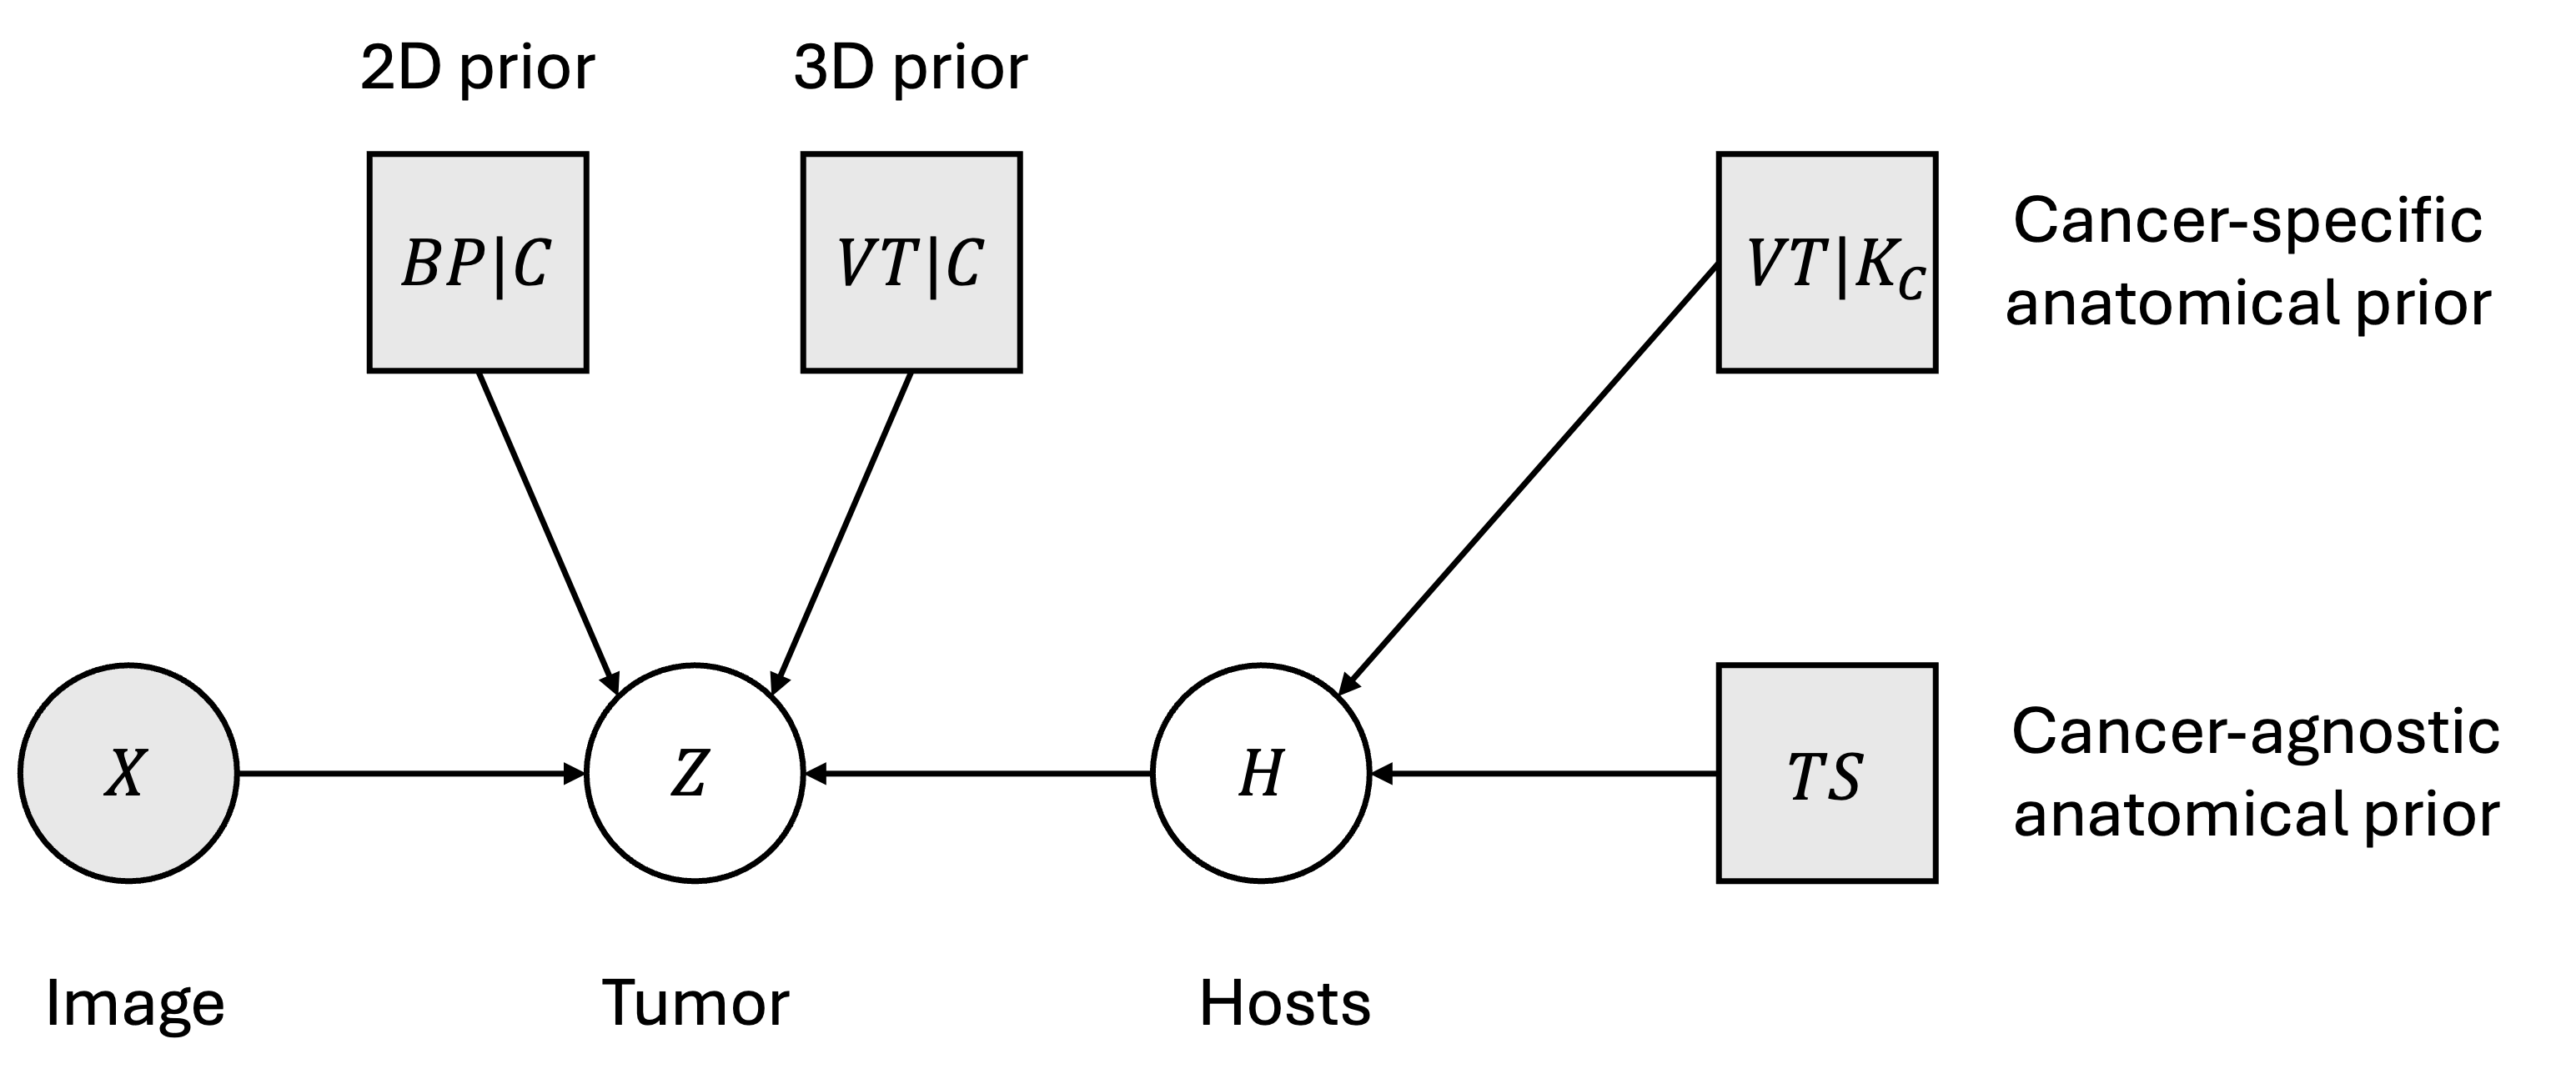
\includegraphics[width=1\linewidth]{figs/PGM.png}}{\fbox{\parbox{0.9\linewidth}{\centering figs/PGM.png not found}}}
    \caption{Conditional probabilistic anatomical reasoning. Each tumor candidate needs two kinds of reasoning, both grounded
    in the image: \emph{host} (which organ it belongs to, and that organ's normal tissue) and \emph{tumor} (whether it is a
    tumor and what its extent is). The host and its normal tissue are inferred first; the tumor is tested against expert
    likelihoods given them.}
    \label{fig:pgm}
\end{figure}

\paragraph{Anatomy.} Organ masks are not taken at face value. Each mask receives a confidence
$\mu(A_{k,o})\in\{0,\tfrac12,1\}$ from the organ--organ relations of $K$: $0$ for a corrupt or impossible mask, $\tfrac12$
for a mask that violates a normal-anatomy expectation that disease can cause, $1$ otherwise. Disagreement between agents is
kept: each organ has a \emph{core}, an \emph{uncertain boundary} and \emph{contested} regions,
\begin{equation}
\label{eq:organ_reference}
\hat H_o=\textstyle\bigcap_{k:\,\mu(A_{k,o})=\mu^{\max}_o}A_{k,o}\setminus\bigcup_{o'}C_{o,o'},\qquad
B_o=\Bigl(\textstyle\bigcup_{k:\,\mu(A_{k,o})>0}A_{k,o}\Bigr)\setminus\bigl(\hat H_o\cup\textstyle\bigcup_{o'}C_{o,o'}\bigr),
\end{equation}
where $C_{o,o'}$ is the overlap of masks of two organs that $K$ does not relate by containment; the territory is
$\Theta_o=\hat H_o\cup B_o\cup\bigcup_{o'}C_{o,o'}$. An expected organ without a usable mask is \emph{unsegmented} and
represented by its knowledge-base region (where it could lie); an organ mostly outside the scan is out of view and is not a
host. The anatomy is a deterministic function of the organ masks and $K$, and is \emph{cut} from the tumor model
\cite{liu2009modularization,plummer2015cuts,jacob2017better}: tumor inference never reshapes an organ.

\paragraph{Set-based units.} Reasoning acts on sets produced by the agents, never on redrawn voxels.
A \emph{claim} is a connected component of one agent's tumor mask from one prompt. An \emph{anchor} $a$ is a component of
the voxels claimed by at least two agents (\emph{two-agent anchor}), or a component of one agent's claims that overlaps no
two-agent anchor (\emph{single-agent anchor}). The \emph{outlines} $\Omega_a$ of $a$ are the claims that overlap it; a part
joined to $a$ only through a narrow neck becomes an anchor of its own (a \emph{lobe}), so support is not transferred along
a bridge. A \emph{lesion} $L$ groups anchors within $10$\,mm of each other. Its \emph{host candidates} $\mathcal{H}_L$ are the
expected hosts in view and any segmented organ to which the anatomy points (closer to the lesion than every expected host,
or holding the largest share of it). Details are in Appendix~\ref{sec:tumor_details}.

\paragraph{Formulation.} For each anchor we infer its host $h_a\in\mathcal{H}_{L_a}$, whether it is a tumor ($z_a$), and its
extent $\xi_a$, chosen from candidate extents built from its outlines,
\begin{equation}
\label{eq:extents}
\mathcal{X}_a=\Bigl\{\,a,\;\;\omega\ (\omega\in\Omega_a),\;\;U_a=\textstyle\bigcup_{\omega\in\Omega_a}\omega,\;\;
U_a\setminus\bigcup_{o\notin\mathcal{H}_{L_a}}\hat H_{o}\Bigr\},
\end{equation}
from the agreed core, through each agent's reading, to their union with and without its leaks into organs that are not
hosts. With $N$ the normal model (the host and its normal tissue) and $T$ the tumor model (existence and extent), the
target is
\begin{equation}
\label{eq:conditional_joint}
p(T,N\mid c_a,X)=p(T\mid N,c_a,X)\;p(N\mid c_a,X),
\end{equation}
with $c_a=(a,\Omega_a,\mathcal{H}_{L_a})$. The two factors are treated according to what expert annotations can estimate.

\emph{Normal model.} The host is inferred from anatomy alone by a choice model over the candidates,
\begin{equation}
\label{eq:normal_model}
P(h\mid L)=\frac{\exp\bigl(\beta^\top\phi_h(L)\bigr)}{\sum_{h'\in\mathcal{H}_{L}}\exp\bigl(\beta^\top\phi_{h'}(L)\bigr)},
\end{equation}
with compatibility features $\phi_h$ (overlap with core and territory, boundary contact, position, mask confidence, distance;
Eq.~\eqref{eq:compat}) and weights $\beta$ fitted on expert tumors of known origin. Because the site of a tumor often cannot
be settled from the image, the host is reported as a \emph{credible set} $\mathcal{S}_L$, the smallest set of candidates
with probability at least $1-\alpha$. The normal tissue $\mathcal{N}_h$ of a host is its core without any agent's claim. The image does not re-rank the hosts:
evidence is computed against each host's own normal tissue, so evidence under different hosts concerns different data.

\emph{Tumor model.} How often an agent's candidate is a tumor depends on the agents, which are not run on expert data, so
existence is not given a posterior but \emph{tested}. Under host $h$, the existence evidence $E^{\mathrm{ex}}_a(h)$ has
likelihood ratio
\begin{equation}
\label{eq:likelihood_ratios}
\Lambda^{\mathrm{ex}}_a(h)=\frac{p\bigl(E^{\mathrm{ex}}_a(h)\mid T,h\bigr)}{p\bigl(E^{\mathrm{ex}}_a(h)\mid N,h\bigr)},
\end{equation}
with both likelihoods estimated as frequencies on expert data: over expert tumors and their partial cores, and over expert
normal structures of $h$'s organ class that an agent can mistake for a tumor. An outcome \emph{rules out} a tumor if
$p(o\mid T,h)\le\alpha<p(o\mid N,h)$ and \emph{confirms} one if $p(o\mid N,h)\le\alpha<p(o\mid T,h)$; other outcomes
are neutral. At most a fraction $\alpha$ of expert tumors is thus ruled out, and at most a fraction $\alpha$ of expert normal
structures is confirmed. The agents'
support enters as an ordinal \emph{support level} $\ell_a\in\{0,1,2\}$: $2$ for two agents and $1$ for one, minus one for each
anatomical warning signal (e.g.\ a host-prompt claim outside its host, a flat claim, a distant lesion without site
agreement). No probability is attached to $\ell_a$, because agent reliability cannot be estimated on expert data. The two are
combined by Table~\ref{tab:decision}; a conflict gives \emph{uncertain}, so an anchor is never rejected against two agents, nor
accepted against the image, without review. Finally, the extent of an accepted anchor maximizes an extent prior
\begin{equation}
\label{eq:extent_prior}
w^0_a(\xi)\;\propto\;\psi\bigl(\log\tfrac{|\xi|}{|a|}\bigr)\prod_{f\in F(\xi)}\eta_f,
\end{equation}
where $\psi$ is a parsimony term over the volume ratio, learned on expert tumors with simulated agent outlines, and
$\eta_f\le1$ would penalise anatomical flags $f$ (leak, organ overlap); the flag factors are currently set to $1$, because
their fitted values depended on how the outlines were simulated (Appendix~\ref{sec:tumor_details}).

\begin{table}[t]
\centering\small
\caption{Stage-1 decision from the support level $\ell$ and the existence test at level $\alpha$.}
\label{tab:decision}
\begin{tabular}{lccc}
\hline
Support level & Confirms & Neutral & Rules out\\
\hline
$\ell=2$ (two agents, no warning signal) & accept & accept & uncertain\\
$\ell=1$ & accept & uncertain & reject\\
$\ell=0$ & uncertain & reject & reject\\
\hline
\end{tabular}
\end{table}

\paragraph{Image grounding.} Agents outline what looks locally abnormal, so local contrast cannot separate a tumor from the
normal structures an agent mistakes for one. Existence evidence therefore uses only properties the agents do not model and
that transfer from expert data to agent candidates: \emph{context} (whether the candidate's deviation from its host's normal
tissue stays closed or continues into the host), \emph{internal structure} (spatially structured heterogeneity) and
\emph{geometry} (elongation). Contrast only decides whether the context test applies. The signs are combined into one
outcome, tumor-like, organ-like or uncertain (Eq.~\eqref{eq:tree}); evidence that cannot be computed is marginalised.
The signs, thresholds and likelihood tables are given in Appendix~\ref{sec:grounding_details}.

\paragraph{Inference.} Inference follows Eq.~\eqref{eq:conditional_joint} in one pass, without iteration or feedback:
(1)~for each lesion, $P(h\mid L)$, the credible set $\mathcal{S}_L$ and the normal tissue of each candidate; a lesion farther
than $10$\,mm from every credible host has an unknown host and is at most uncertain; (2)~for each anchor and each
$h\in\mathcal{S}_L$, the existence test and the decision of Table~\ref{tab:decision}, which must agree across the credible
set, otherwise the anchor is uncertain; (3)~for an accepted anchor, the extent $\hat\xi_a=\arg\max_\xi w^0_a(\xi)$. The
stage-1 segmentation is the union of the chosen extents, each reported with its host credible set and role (primary, local
invasion, distant).

\subsection{Stage 2: voxel-wise Bayesian tumor segmentation}
\label{sec:stage2}
Stage~1 reasons globally, over relations between tumor units and organs, and its extents are choices among the agents'
outlines. Stage~2 works locally on every accepted and uncertain lesion: where exactly the tumor is, which voxels the agents
included wrongly or missed, and how the tumor is composed. It reads only stage-1 outputs, never the agents' masks, so it is
agent-agnostic. The host is now \emph{known with uncertainty}: $P(h\mid L)$ over $\mathcal{S}_L$ is a fixed prior, and the
anatomy stays cut. No voxel is fixed to tumor in advance: the mask is latent, with a prior learned from expert data.

\paragraph{Stage-1 extent marginal.} The candidate extents and their prior are summarised per voxel,
\begin{equation}
\label{eq:qv}
q^a_v=\sum_{\xi\in\mathcal{X}_a}w^0_a(\xi)\,\mathbf{1}[v\in\xi],\qquad
q^L_v=1-\prod_{a\in L}\bigl(1-q^a_v\bigr),
\end{equation}
which is $1$ on the anchors, decreases outward and is $0$ beyond every candidate, so stage~2 does not commit to the chosen
extent.

% Joint formulation drafted 26 Oct 2026 (Claude, with the user) after the tail study (Appendix C); implemented the same night
% (features D = 4, per-class MAP nu under the cell priors; pancia_kb/stage2/features.py, vb.py, run.py, nuprior.py).
\paragraph{Joint model.} On a region $R_L$ around the lesion that includes all its credible hosts (Eq.~\eqref{eq:roi}),
each voxel has features $y_v=\bigl(I_v,\,\partial_1 I_v,\,\partial_2 I_v,\,\nabla^2_{\sigma}I_v\bigr)$: the normalised intensity,
its first differences along the two in-plane axes and the in-plane Laplacian of Gaussian ($\sigma=1$\,mm), that is,
statistics of order $0$, $1$ and $2$; derivatives describe spatial change and depend less on the imaging protocol than the
intensity level. Each voxel has a label $Z_v\in\{0,1,\dots,K_{\max}\}$, background or one of $K_{\max}$ tumor components, with
tumor indicator $t_v=\mathbf{1}[Z_v\ge1]$, and a latent scale $u_v>0$. Given the stage-1 outputs $\mathcal{O}_1$ (the extent
marginal, the chosen extent, the credible hosts with $P(h\mid L)$, and the anatomy), the joint distribution is
\begin{equation}
\label{eq:joint}
\begin{aligned}
p(y,Z,u,\theta,\boldsymbol\rho,\boldsymbol\nu,\omega\mid\mathcal{O}_1)={}&
\underbrace{\textstyle\prod_{v}p(y_v\mid Z_v,u_v,\theta)\,p(u_v\mid Z_v,\boldsymbol\nu)\;p(\theta)}_{\text{appearance}}\\
&\times\underbrace{p(Z\mid\pi,\boldsymbol\rho,\omega)\,p(\omega)}_{\text{host and spatial priors}}\;
\underbrace{p(\boldsymbol\rho)\,p(\boldsymbol\nu)}_{\text{intra-tumoral prior}}.
\end{aligned}
\end{equation}
Three kinds of prior knowledge enter one posterior. The \emph{host prior} is inter-tumoral: a tumor is compared with the normal
tissue of its credible hosts, so two tumors in one host are compared through it. The \emph{spatial prior} says where tumor
lies relative to the agents' outlines and the anatomy. The \emph{intra-tumoral prior} describes how a tumor is composed: its
components and their heterogeneity. They are inferred jointly because which voxels are tumor, how they group into components
and how heavy-tailed each component is depend on one another.

\emph{Spatial prior.} Tumors are not spatially homogeneous: they arise in particular organs, extend beyond the agents'
outlines by characteristic distances and invade neighbours. The prior probability of tumor is
\begin{equation}
\label{eq:spatial_prior}
\pi^L_v=P(t_v=1)=\sum_{h\in\mathcal{S}_L}P(h\mid L)\;\sigma\bigl(\eta^\top\psi_v(h)\bigr),
\end{equation}
a mixture over the credible hosts, where $\psi_v(h)$ is a fixed basis of $q^L_v$, the signed distance to the chosen extent,
the territory of $v$ relative to $h$ and its depth inside that organ. Lesions whose regions overlap are inferred jointly, with
$\pi_v=1-\prod_L(1-\pi^L_v)$. The weights $\eta$ are fitted on expert tumors with simulated agent outlines that over- and
under-segment; every simulated outline surrounds a real tumor, so Eq.~\eqref{eq:spatial_prior} is a prior on \emph{extent}
given that the lesion is a tumor, not on existence. It gives positive probability beyond the agents' outlines, which is what
allows recall. Neighbouring tumor indicators are coupled by a Potts term with latent edge weights \cite{gao2023bayeseg},
\begin{equation}
\label{eq:mrf}
\begin{aligned}
p(Z\mid\pi,\boldsymbol\rho,\omega)\;&\propto\;\textstyle\prod_{v}\bigl(\pi_v\rho_{Z_v}\bigr)^{t_v}(1-\pi_v)^{1-t_v}
\,\prod_{v\sim w}\exp\bigl(-\omega_{vw}\,s_{vw}\,\mathbf{1}[t_v\ne t_w]\bigr),\\
\omega_{vw}&\sim\mathrm{Gamma}(a_\omega,b_\omega),
\end{aligned}
\end{equation}
where $s_{vw}$ scales a pair by its physical distance. Where the image separates two voxels the posterior weight is small, so
the boundary follows image contrast rather than a fixed smoothness.

\emph{Appearance.} Appearance does not transfer across scans (contrast phase, MR scale, sequence and scanner differ), so its
parameters $\theta$ are inferred within each scan, with weak Normal--Wishart priors from the scan's own voxels. Every class
$j$, tumor component $k=1..K_{\max}$ or background class $c\in\mathcal{C}$, has a Student-$t$ likelihood written as a scale
mixture,
\begin{equation}
\label{eq:appearance}
y_v\mid Z_v{=}j,u_v\sim\mathcal{N}\bigl(\mu_j,(u_v\Lambda_j)^{-1}\bigr),\qquad u_v\mid Z_v{=}j\sim\mathrm{Gamma}\bigl(\tfrac{\nu_j}{2},\tfrac{\nu_j}{2}\bigr),
\end{equation}
where the background mixes its classes with weights $\lambda_{v,c}$ (the organs whose territories meet the region and three
generic classes). One scale $u_v$ is shared by all features: a voxel atypical for its class is atypical at every order at
once, which fits expert data better than a separate scale per order (Appendix~\ref{sec:stage2_details}).

\emph{Intra-tumoral prior.} Tumor and normal tissue use the same likelihood family with different priors on the tail weight,
keyed by the modality $\mu\in\{\mathrm{CT},\mathrm{MR}\}$ and the knowledge-base \emph{tissue class} $\kappa$ of the host:
parenchymal (solid organs and glands), hollow (a lumen or cavity with its wall and contents) or aerated (lung and airways),
\begin{equation}
\label{eq:nu_prior}
\begin{aligned}
\log\nu_k^{-1}&\sim\textstyle\sum_{h\in\mathcal{S}_L}P(h\mid L)\,\mathcal{N}\bigl(m^T_{\mu,\kappa(h)},(s^T_{\mu,\kappa(h)})^2\bigr), && k=1..K_{\max},\\
\log\nu_c^{-1}&\sim\mathcal{N}\bigl(m^N_{\mu,\kappa(c)},(s^N_{\mu,\kappa(c)})^2\bigr), && c\in\mathcal{C}.
\end{aligned}
\end{equation}
The classes describe imaging physics, not cancer types: heavy tails arise at interfaces with air, lumen contents or fat, which
depend on the host tissue rather than on the cancer's identity, so the key applies to any cancer. The priors are estimated
hierarchically on expert tissue components of tumors and of the normal tissue around them, with sites weighted equally; a
tissue class without expert tumors (bone, lymph nodes, fat, muscle, brain), an empty cell and the generic background classes
take the pan-cancer prior, whose spread includes the variation between cells (Appendix~\ref{sec:stage2_details}). The tail weight is
not what separates tumor from normal tissue: on expert data, whole normal regions are heavier-tailed than tumors, because they
mix vessels, fat, air and organ edges, while single components of tumor and normal tissue have similar tails
(Appendix~\ref{sec:stage2_details}). Tumor versus normal is decided by the host and spatial priors; $\nu_k$ describes the
heterogeneity within a tumor tissue. The component weights follow a sparse Dirichlet, $\boldsymbol\rho\sim\mathrm{Dir}(\alpha_0)$
with $\alpha_0<1$, so the number of components (substructures such as solid tissue and necrosis) is inferred per lesion up to
$K_{\max}=4$.

\paragraph{Inference and outputs.} The posterior is approximated by mean-field variational Bayes,
$q(Z)\,q(u)\,q(\theta)\,q(\boldsymbol\rho)\,q(\omega)$, with closed-form updates \cite{gao2023bayeseg}; each $\nu_j$ is a point
estimate maximising the lower bound plus its log prior (Eq.~\eqref{eq:nu_update}). Inference starts from $q(t_v=1)=q^L_v$. The
outputs are the voxel tumor posterior $p_v=q(t_v=1)$; the refined tumor $\hat Z_L$, the components of $\{p_v\ge\tfrac12\}$ that
meet an anchor of $L$; the component posteriors, an intra-tumoral substructure map, with each component's tail weight $\nu_k$;
and an atypicality map $1/\mathbb{E}[u_v]$, which marks voxels unlike the rest of their component (for example calcification,
haemorrhage or vessels inside a tumor). Relative to the chosen extent, $\hat Z_L$ gives the voxels trimmed from and recalled
beyond the agents' outlines; components that meet no anchor are reported as new candidates without a decision.

\paragraph{Control.} Because no voxel is fixed, the image may prefer background alone. On the anchor neighbourhood $N_L$
we compute the approximate Bayes factor
\begin{equation}
\label{eq:stage2_bf}
\log\widehat{\mathrm{BF}}_L=\mathcal{L}_{N_L}(\text{tumor and background})-\mathcal{L}_{N_L}(\text{background only}),
\end{equation}
with $\mathcal{L}$ the variational lower bound and both models given the same flexibility. If $\widehat{\mathrm{BF}}_L<1$
the lesion is flagged and its stage-1 extent is kept. The stage-1 decision is not changed.

%====================================================================================================================
\section{Experiments and Results}
\label{sec:results}
% Updated 18 Oct 2026 for ledger v7 + grounding G1. Numbers marked [TBD] are filled after the expert-data checks and the
% frozen TCGA run. Stage is reported only; nothing is tuned on stage. TCGA has no tumour annotation: it serves visual checks,
% blind ratings and reporting only; expert data is the only quantitative validation.

\subsection{Data}
We use the public TCGA radiology collections of The Cancer Imaging Archive (TCIA). The cohort contains 3{,}291
baseline-study series (1{,}407 CT, 1{,}884 MR) from 15 cancer types: BLCA, BRCA, CESC, COAD, ESCA, KICH, KIRC, KIRP,
LIHC, LUAD, LUSC, OV, PRAD, STAD and UCEC. TCIA states that only the baseline study precedes surgery, and post-surgical
studies cannot be identified, so all evaluations use the baseline study only. The stage-evaluation scope is restricted
to baseline series with the primary organ in the field of view: 3{,}116 series from 942 patients. Scans graded \emph{exclude} by image quality control (Appendix~\ref{sec:qc_details}) are removed and reported with their reason ([TBD] series); \emph{degraded} scans ([TBD]) are kept without image grounding. Clinical stage comes
from the TCGA clinical records. No voxel-level tumour annotation exists for this cohort, so TCGA is used only for visual
inspection, blind ratings of candidates and the stage-free yardsticks below; no likelihood, prior or threshold is estimated
on it. Outputs of a pilot of 152 TCGA series were inspected visually for implementation errors only. The corrections that
followed (the anatomy checks for small or multi-component organ masks, the laterality check, the grading of dedicated
protocols with little anatomy in view, the knowledge-base region of an unsegmented organ, and the candidacy of organs
outside $\mathcal{H}_C$) fixed errors and estimated no likelihood, prior or threshold; the pilot series are reported
separately.

The likelihoods of image grounding are built only from public expert annotations: tumour masks of the R2Seg collections
(bladder, breast, cervix, colon, kidney, liver, lung, pancreas, prostate and uterus, including benign uterine fibroids;
[TBD] masks) and normal anatomy of
TotalSegmentator CT (v3.0, scans without pathology) and MR (v3.0, scans from the original release source; scans indexed from the
Imaging Data Commons, which hosts TCIA collections, are excluded to avoid overlap with the evaluation cohort), adults only ([TBD] scans). Neither enters the evaluation cohort.

\subsection{Implementation}
The tumour agents are BiomedParse (2D) and VoxTell (3D promptable); the anatomy agents are TotalSegmentator and VoxTell. The
knowledge base has 204 entities and 433 relations (v0.5.8). Host and tumour reasoning are deterministic set operations.
The likelihood tables of image grounding and the outcomes that rule out or confirm a tumor at level $\alpha$, the
compatibility weights $\beta$ and the parsimony term $\psi$ are estimated on expert data (the flag factors $\eta_f$ are set to
$1$) and frozen
before any TCGA result (Appendix~\ref{sec:grounding_details}); the remaining design choices (the ordinal support levels, the
decision table, the error level $\alpha$ and the geometric constants) and their sources are listed in Table~\ref{tab:constants} (Appendix~\ref{app:constants}). The whole cohort was processed on a CPU cluster in [TBD] hours.

\subsection{Evaluation without voxel ground truth}
\label{sec:eval_protocol}
Without voxel annotations, we use stage-free yardsticks that a correct segmentation must satisfy. All are computed on
the baseline study only:
\begin{itemize}
  \item \emph{spread}: the median $|\log(v/\tilde v)|$ of the index-lesion volume $v$ across the series of one study,
  where $\tilde v$ is the study median;
  \item \emph{cross}: the share of same-study series pairs whose sizes differ by at least one RECIST progression step;
  \item \emph{disagree}: the share of series whose index lesion is not the study's majority lesion;
  \item \emph{miss}: the share of baseline series with no measurable lesion (the primary tumour is present before
  surgery).
\end{itemize}
In addition, [TBD] agent candidates were rated blind by a reader (tumour, not tumour, unsure); these ratings measure the
precision of image evidence against a candidate and the share of rated tumours it rejects. The patient-median Spearman
correlation with T and overall stage is reported for reference only. No parameter, rule or threshold is selected on stage
or on the ratings.

\subsection{Validation of image grounding on expert data}
\label{sec:results_expert}
Because TCGA has no tumour annotation, the reasoning is validated where truth is known, on a testbed built from expert
data only (R2Seg collections with expert organ and tumour labels: kidney, liver, pancreas, lung, cervix and prostate; and
TotalSegmentator normal anatomy). Agents are not run on these data; instead, agent-like candidates are simulated from the
expert masks: cores (partial sub-regions and three-slice cuts), outlines (exact, dilated by $3$--$5$\,mm, grown into the
host's own parenchyma, leaking into a neighbour, organ-sized, and with a false lobe joined by a thin bridge), normal
candidates (vessel and bowel tube segments, organ parts and edges, salient intra-organ structures), and perturbed organ
masks (leaks, merges, missing parts, the tumour included in the organ, and the true host unsegmented and represented by
its knowledge-base region, with the regions of its neighbours as negatives). Every estimate is held out (leave one R2Seg
collection out; two folds of TotalSegmentator). We report: (i)~existence: for each $\alpha$, the held-out rates at which expert tumour cores are ruled out and expert normal
candidates are confirmed, overall and for candidates below $3$\,ml;
(ii)~host: top-1 attribution and the coverage and size of the host credible set of expert tumours among their true and
neighbouring organs, and how often the credible set holds both organs of synthetic invasion cases (an expert tumour joined
to a band of its labelled neighbour), separately for intraparenchymal,
straddling and exophytic tumours and under perturbed organ masks; (iii)~extent: how often $\hat\xi$ is the extent closest to
the expert mask, its Dice, its volume ratio, and how often it grows into host parenchyma; (iv)~sensitivity to $\alpha\in\{0.01,0.05,0.10\}$, to $\tau$ and the host tolerance $\delta$, and to the image
quality-control thresholds. [TBD]

\subsection{Effect of image-grounded reasoning}
\label{sec:results_r2}
Host and tumour reasoning are identical with and without image grounding ($\Lambda=1$), so the comparison isolates it.
Table~\ref{tab:r2_by_type} reports, per cancer type, the anchors accepted, uncertain and rejected by the support levels alone (every
outcome neutral) and with the existence test; anchors whose host credible set holds more than one organ; overrides of the
decision policy;
lesions whose host joined the expected list or is unknown; and the volume between the anchor and the union of outlines that the chosen extents keep. [TBD: main pattern.] On the rated candidates, image evidence against a
candidate is correct in [TBD]\,\% and rejects [TBD]\,\% of rated tumours.

\begin{table}[t]
\centering\small
\caption{Image-grounded reasoning per cancer type (baseline series). \emph{Reasoning only}: accepted anchors with
every outcome neutral. \emph{Rejected}/\emph{recovered}: anchors whose decision the existence test changed. \emph{Host
set}: anchors whose host credible set holds more than one organ. \emph{Override}: primary-not-detected overrides.}
\label{tab:r2_by_type}
\setlength{\tabcolsep}{4pt}\footnotesize
\begin{tabular}{lrrrrrrr}
\hline
Cancer & Series & \shortstack{Reasoning\\only} & Grounded & Rejected & Recovered & \shortstack{Host\\set $>1$} & Override\\
\hline
\multicolumn{8}{c}{[TBD]}\\
\hline
All & 3{,}291 & & & & & & \\
\hline
\end{tabular}
\end{table}

\subsection{Baseline yardsticks}
\label{sec:results_yardsticks}
Table~\ref{tab:yardsticks} compares BiomedParse alone, VoxTell alone, reasoning only, and the full model on the
yardsticks of Section~\ref{sec:eval_protocol}. [TBD: main finding, stated without reference to stage.]

\begin{table}[t]
\centering\small
\caption{Stage-free yardsticks on 3{,}116 baseline series (942 patients). The Spearman $\rho$ with T stage is reported
only and was not used for any choice.}
\label{tab:yardsticks}
\begin{tabular}{lrrrrr}
\hline
Method & Spread & Cross (\%) & Disagree (\%) & Miss (\%) & $\rho_T$ (reported)\\
\hline
BiomedParse & & & -- & & \\
VoxTell & & & -- & & \\
Reasoning only & & & & & \\
Full model & & & & & \\
\hline
\end{tabular}
\end{table}

\subsection{Qualitative results}
[TBD: Fig.~\ref{fig:grounding} to be regenerated with the G0 outputs: an anchor with its outlines and priors, its evidence
outcome, test result and likelihood ratio per host in its credible set, and the chosen extent.]
\begin{figure*}[t]
    \centering
    \IfFileExists{figs/r2_grounding_g0.pdf}{\includegraphics[width=\linewidth]{figs/r2_grounding_g0.pdf}}{\fbox{\parbox{0.9\linewidth}{\centering figure to be regenerated}}}
    \caption{Image-grounded reasoning on a public TCGA scan. Left: anchors (filled), outlines of each agent and the reasoning
    priors. Middle: evidence state and likelihood ratio of each extent under each host. Right: accepted tumours with their
    chosen extents. [TBD]}
    \label{fig:grounding}
\end{figure*}

\subsection{Ablation}
\label{sec:ablation}
[TBD, on the expert testbed and with the columns of Table~\ref{tab:r2_by_type} on TCGA: (i)~numerical support priors
($\pi_{\text{two}}\in\{0.75,0.9\}$, $\pi_{\text{single}}=0.5$, odds factor $1/3$ per warning signal, thresholds $0.75/0.25$)
instead of the support levels and the test at $\alpha$; (ii)~the knowledge-base host weights ($1/0.3/0.15$) instead of equal
weights; (iii)~each evidence component removed in turn (context, internal structure, geometry); (iv)~no parsimony term
$\psi$ or flag factors $\eta_f$, and the extent evidence added; (v)~flagged outlines removed from $\mathcal{X}_a$ instead of
penalised; (vi)~binary touch instead of the compatibility features; (vii)~a ruled-out two-agent anchor rejected instead of
uncertain; (viii)~$\alpha\in\{0.01,0.05,0.10\}$.]

\subsection{Limitations}
\begin{itemize}
  \item Image quality control relies on what the anatomy agents can segment; a scan whose organs fail for reasons other than quality (unusual anatomy, post-surgical change outside the primary, or a dedicated protocol with little anatomy in view) may be graded degraded.
  \item There is no voxel-level ground truth, so accuracy is assessed through stage-free yardsticks, expert data and
  blind ratings of candidates.
  \item In stage~1, image evidence decides existence and chooses among the agents' outlines; boundaries are redrawn only in
  stage~2. A tumour that no agent proposes is not localized, and stage~2's prior far beyond the agents' outlines is learned
  only from scans with several tumours.
  \item Agent agreement cannot be calibrated on expert data, because the agents are not run there; it enters as ordinal
  support levels, and existence is tested rather than given a posterior probability.
  \item On expert data the existence test rules out far more often than it confirms: few outcomes confirm a tumour of
  $3$\,ml or more, so acceptance of larger candidates rests mainly on agent agreement.
  \item The site of a tumour often cannot be decided from the image; the host is reported as a credible set, and the image
  does not re-rank hosts.
  \item The extent is chosen by a prior learned on expert data, not by image evidence, which did not improve the choice
  of extent on held-out expert data.
  \item Invasion is represented only between the primary organ and its local-invasion organs in $K$; the host testbed
  contains intraparenchymal expert tumours only.
  \item The expert three-slice cores of the existence tables are cut on the common $\sim5$\,mm grid; agent cores of three
  native slices are thinner, and on the testbed such cores were ruled out in $21\%$ of cases at $\alpha=0.05$ [to be
  resolved by rebuilding these items at native resolution].
  \item Other or indeterminate lesions are reported but not characterised.
  \item Many agent false positives remain uncertain rather than organ-like: normal sub-structures that resemble tumour
  (intra-organ vessels, renal sinus, bowel loops) are the main confounder, and iso-intense candidates have no context test.
  \item The stage-2 tail-weight prior has no expert tumours of neural, musculoskeletal, haematolymphoid or diffuse tissues
  (brain, bone, muscle, lymph nodes, fat); tumours hosted there receive the pan-cancer prior. Its MR row is estimated mostly on
  T2-weighted scans.
  \item Evidence is weaker on MR than on CT, and hosts without expert normal anatomy (for example ovary and breast) use pooled
  normal tables.
  \item The default distant-site lists do not include brain, and pleura and distant lymph nodes have no anchor in
  the knowledge base, so metastases there are not reported.
\end{itemize}

\section*{Acknowledgments}

Additional information can be given in the template, such as to not include funder information in the acknowledgments section.

\bibliography{modular_refs}

\appendix

\section{Knowledge base and prompt planning}
\label{sec:kb_planning}
\begin{figure}
    \centering
    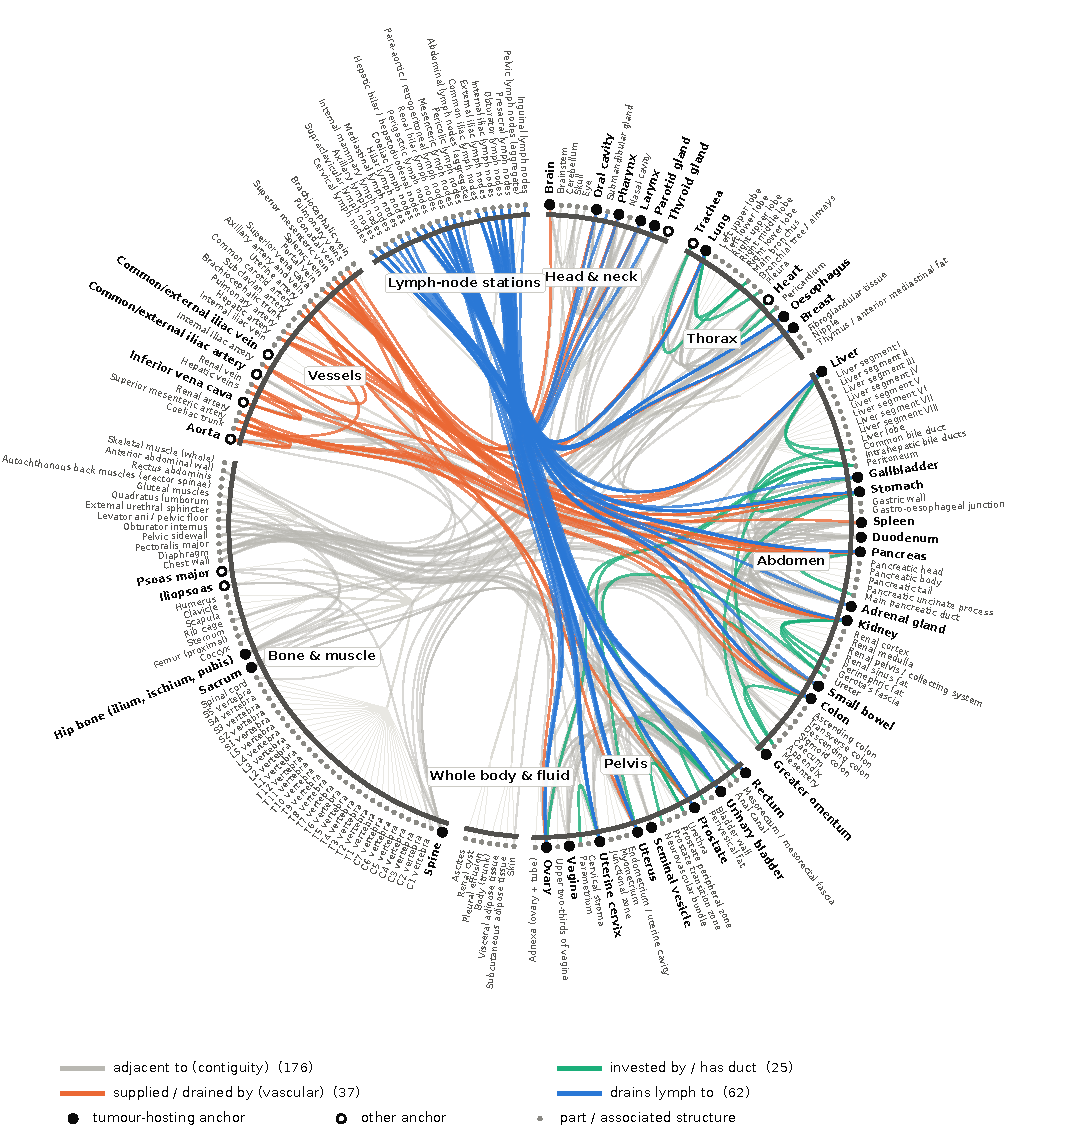
\includegraphics[width=0.9\linewidth]{figs/kb_graph.pdf}
    \caption{Pan-cancer anatomical knowledge graph}
    \label{fig:kb_graph}
\end{figure}

This appendix describes how the anatomical knowledge base $K$ is built once for all cancer types, and how, for each scan,
it is turned into the VT prompt plan $K_C$ of Eq.~\eqref{eq:agents}. $K$ is a curated, image-independent graph;
$K_C$ is a finite list of prompt jobs, and $V_K=f_{\mathrm{VT}}(X,K_C)$ is the stack of masks VT returns for these jobs.
No component of $K$ or of the planner uses patient sex, and no rule or constant is specific to an organ, a cancer type
or a dataset.

\paragraph{Anatomical entities.}
$K$ contains 204 anatomical entities. Each entity has a category (solid organ, hollow organ, gland, bone, vessel,
lymph-node station, muscle, fascia, fat, duct, space, nerve, landmark or region) and a laterality (left, right, midline
or bilateral). It also records how it can be observed: the TotalSegmentator classes that represent it for CT and for
MR, if any; a VT main phrase with up to two aliases, each graded as in-vocabulary, near-vocabulary or
out-of-vocabulary against the published VT training vocabulary; its craniocaudal span between vertebral anchors;
whether it is always present, variably present or absent after common surgery; a typical volume range; and, for CT, a
typical Hounsfield-unit range. Finally, each entity that can host a tumor carries a tumor phrase (for example
\emph{liver tumor}). Thirty-nine entities are \emph{anchors}: structures that TotalSegmentator segments reliably and
that therefore fix the coordinate frame of a scan (vertebrae, major vessels and large organs). Landmarks are tied to
vertebral levels, so that every spatial prior in $K$ is expressed relative to the patient's own skeleton rather than in
millimetres.

\paragraph{Anatomical relations.}
Entities are connected by 433 typed, directed relations. Ten relation kinds are defined, of which nine are used:
\emph{adjacent\_to} (176), \emph{has\_part} (97), \emph{drains\_lymph\_to} (62), \emph{lies\_in} (23),
\emph{supplied\_by} (21), \emph{invested\_by} (16), \emph{drained\_by} (16), \emph{landmark\_for} (13) and
\emph{has\_duct} (9); the tenth, \emph{wall\_of}, is reserved. Each relation kind has a fixed spatial gate and a default
priority. The gate states where the target may lie relative to the source: inside it (\emph{has\_part}), in a shell
around it (\emph{invested\_by}), in a neighbouring box or directional shell (\emph{adjacent\_to}), in a corridor along
a vessel or duct (\emph{supplied\_by}, \emph{drained\_by}, \emph{has\_duct}) or in a body region
(\emph{drains\_lymph\_to}); \emph{lies\_in} and \emph{landmark\_for} carry no gate. Gates are later used to check VT
outputs against structures that are already segmented, and priorities order prompts when the budget is exceeded. The relations encode the anatomy that staging systems refer to: direct extension
into a neighbouring organ, invasion of an investing fascia or fat, and lymphatic drainage to a regional station.

\paragraph{Cancer-type spread sets.}
For each cancer type $C$, $K$ stores the expected host list $\mathcal{H}_C$ (with roles, not weights), which is the host list used in
Appendix~\ref{sec:reasoning_details}. Only two items are specified per cancer type: the primary organ and a list of
distant metastatic sites. Organs at risk of local invasion are not curated; they are
derived automatically as the entities reached from the primary organ by an \emph{adjacent\_to} or \emph{invested\_by}
relation that carries an invasion staging tag, with the relation's side rule for paired organs. A route that ends at a part
no agent segments (for example the sigmoid colon) is mapped to its nearest segmented whole along \emph{has\_part} (the
colon), with the same role; distant sites are mapped in the same way. The reasoning takes this list from $K$; the
planner's use of the initial tumor priors (step~iii below) orders prompts and never removes a host from it. Organs present
in one sex only (uterus, cervix, vagina, ovary, prostate, seminal vesicle) are hosts only where $K$ lists them for the
cancer type: patient sex is not used, so a mask of such an organ cannot be verified and is never added by proximity. Each cancer type also has a short ensemble of tumor phrases (for example \emph{lung cancer}, \emph{lung
tumor}, \emph{lung mass}), and generic templates produce phrases for any host without a curated one. The distant-site lists are user-defined inputs rather than an exhaustive account of metastatic spread. Here we
restrict each list to the most common metastatic sites reported for that cancer type that are also anchors of $K$, and
cancer types without a curated list default to liver, lung, adrenal gland and spine. Head-and-neck anchors (brain, oral cavity,
pharynx, larynx and parotid gland) are part of $K$ but are in no default list, because the body scans considered here
rarely include the head and neck. Sites that are not anchors, such
as the pleura and distant lymph nodes, are not prompted. A user can extend a list, or add an anchor, without changing any other part of the framework, and only the affected cancer types need to be re-planned. The current
base covers 17 TCGA cancer types, plus a CPTAC entry whose cancer type is resolved per case. Adding a new cancer type
therefore requires only its primary organ, its metastatic sites and, optionally, its phrase ensemble; all other
knowledge is shared.

\paragraph{Planning $K_C$ for a scan.}
For a given scan, the planner builds $K_C$ deterministically in a single pass, without calling any segmentation model.
Its inputs are the modality, the cancer type $C$, a summary of the TotalSegmentator output $T$ (which classes are
present, their volumes and their extents), and the initial tumor priors $B_C$ and $V_C$ of Eq.~\eqref{eq:agents}.
It proceeds in five steps.

\emph{(i) Frame.} The vertebrae found in $T$ define a craniocaudal ruler. The landmarks of $K$ are placed on this ruler,
and every entity span is converted to a slice range of the scan. This step also determines which entities lie inside the
field of view.

\emph{(ii) Anchors.} Each anchor is labelled \emph{found} (present in $T$ with a plausible volume and position),
\emph{expected} (inside the field of view but missing from $T$) or \emph{missing} (outside the field of view). Found
anchors give the reference structures against which the gates of later prompts are evaluated.

\emph{(iii) Tumor evidence.} A component of $B_C$ or $V_C$ is \emph{validated} when the two priors agree on it. For each
host $h\in\mathcal{H}_C$ the planner records an evidence level $e_h\in\{0,1,2\}$: $2$ if a validated component lies in
or within a reach of $10$\,mm of $h$, $1$ if a component from one prior does, and $0$ otherwise. It also records the
side of the primary tumor for paired organs. The planning priority of the host is $r_h(1+e_h)$, where $r_h$ ranks its role
(primary $1$, local invasion $0.3$, distant $0.15$); it only orders prompts under the budget and plays no part in
inference. The initial tumor priors therefore influence only the order and the extent of the anatomical
prompts; they never remove a host from $\mathcal{H}_C$.

\emph{(iv) Prompt tiers.} Prompts are generated in four tiers. Tier~0 adds ruler prompts (spine, sacrum, hip bone) only
when $T$ provides neither vertebrae nor fallback landmarks, so that a frame can always be placed. Tier~1 completes the anchors that are expected but missing from $T$, each gated by its
spatial prior. Tier~2 adds \emph{anatomical profiles} by walking the relation graph: two hops from the primary organ,
one hop from each secondary host, and the structures that can be reached from any host with tumor evidence
$e_h>0$. Tier~T contains the tumor prompts: one prompt with the tumor phrase of each host of $\mathcal{H}_C$ inside the
field of view. Tier~T is issued for every such host regardless of the evidence $e_h$, so that a lesion missed by both
initial priors can still be proposed. For the same reason, when the initial VT tumor mask is empty or smaller than
$0.5$\,ml, the cancer-type phrase ensemble is added for the primary organ. This is a wording ensemble for the same
model, not a second rater: the initial and prompted VT outputs are counted as one model in tumor reasoning.

\emph{(v) Budget.} The plan is limited to $80$ prompts. Tiers~0, 1 and T are protected; only tier~2 is trimmed, lowest relation
priority first, with items derived from a host given a one-step priority boost.

The output $K_C$ is the list of prompt jobs that survive the budget. Each job records the entity, its side, the phrases to
issue (the main phrase and its first two aliases), its tier, its gate, and, for tumor prompts, the host and its
role. VT is run once per scan on the full volume with all jobs of $K_C$; there is no re-planning after inference.
For each job, the masks of its three phrases are fused by voxel-wise majority (at least two of three). The gate is then
applied as an output filter: each connected component of the fused mask is kept only when at least $80\%$ of its
voxels lie inside the region allowed by the gate. A completion structure that is empty after filtering is recorded as
absent when $K$ marks it as variable or removable by surgery, and as not found otherwise. The kept organ masks form $V_K$, which enters the organ references
$\hat H_o$. The masks of the tier-T jobs are tumor proposals; they are added to VT's tumor masks $V_C$ as host-prompt
claims, each tagged with its prompted host, and are subject to the same host, tumor and image reasoning as every other claim.

Two properties of this construction matter for the reasoning that follows. First, although $K$ is independent of the
image, $K_C$ is not: it depends on $T$ through the frame and the anchors, and on the initial tumor priors through the
evidence levels. This dependence is restricted to which structures are prompted and in what order, so it changes the
coverage of $V_K$ but not the meaning of any mask. Second, because tier~T prompts every plausible host whether or not it
contains a tumor, VT is regularly asked to segment a tumor that is absent. Its output for such a prompt can be a false
positive inside the prompted host or elsewhere in the scan. These proposals are therefore treated as priors only, and
whether they are accepted is decided by image grounding
(Appendix~\ref{sec:grounding_details}).

\section{Stage-1 reasoning details}
\label{sec:reasoning_details}
% From the 22 Oct text (stage 1 = ledger v8.4), moved here 26 Oct 2026. Constants and their sources: Table~S1 (Appendix D).

All operations are per scan on the native voxel grid. Distances are Euclidean in millimetres. The \emph{acquisition axis}
is the axis with the largest voxel spacing when the ratio of largest to smallest spacing is at least $1.5$, and the
superior--inferior axis otherwise; slice-wise operations use the plane orthogonal to it. No rule names a cancer type or an
agent, no constant is tuned on clinical endpoints, and patient sex is never used. The source of every constant (expert
data, knowledge base, or design choice) is listed in Table~\ref{tab:constants} (Appendix~\ref{app:constants}); design constants are few and their
sensitivity is reported.

\paragraph{Relations and roles.} Host and tumor reasoning are set-based relational checks against $K$. $K$ stores
organ--organ relations $\mathcal{R}_{AA}$ (containment: \emph{has part}, \emph{lies in}, \emph{invested by};
\emph{adjacent to} with contact and direction; spatial priors with direction and distance; and, by default, disjointness of
organs it does not relate by containment) with unary organ attributes, and tumor--organ relations $\mathcal{R}_{TA}$ (inside,
straddling or touching an organ, extending into an adjacent organ, lying at a cancer-specific distant site, being or containing
an organ, lying in an organ that is not a host of the cancer type). \emph{Host reasoning} evaluates $\mathcal{R}_{AA}$ between
anatomy masks and gives the anatomy (mask confidences, organ states, cores, boundaries and contested regions); it reads anatomy
masks only, so the anatomy stays cut. \emph{Tumor reasoning} evaluates $\mathcal{R}_{TA}$ between tumor units and the anatomy
and gives the host candidates, the compatibility features, the anatomical flags, the support levels and the extent prior.
Neither uses image intensities. Only what is impossible is decided early (a corrupt agent output is removed; an organ out of
view is not a host); everything else that is anatomically unsupported lowers the support level or flags a unit, and the image
can overturn it. Silence of another agent is evidence neither for nor against a candidate. The roles $\kappa_h$ of the expected
hosts enter inference only through the site-agreement warning signal of a distant host and the local-invasion explanations
below; otherwise they are attached to a host after inference. Because the cancer is confirmed and the scans precede surgery, a
primary tumor exists in the scan; this is represented at scan level by the decision policy and does not make any particular
candidate near the primary organ the primary tumor.

\paragraph{Order of computation.} (0) image quality control; (1) host reasoning: mask confidence, organ states, cores,
boundaries and contested regions; (2) claims, anchors, lobes and outlines; (3) host candidates, anatomical compatibility
and lesions; (4) anatomical flags, support levels and extent prior; (5) normal tissue and image evidence; (6) one-pass
conditional inference; (7) decision policy.

%--------------------------------------------------------------------------------------------------------------------
\subsection{Image quality control}
\label{sec:qc_details}
Image grounding needs an image in which the anatomy agents can delineate normal organs. Each scan receives a state
$Q\in\{\text{good},\text{degraded},\text{exclude}\}$ before reasoning. Let $\mathcal{E}$ be the organs the planner expects in
view (obligatory presence, at least half of its vertebral span in the frame). An expected organ \emph{fails} if an agent
segmented it but every mask of it is infeasible ($\mu=0$). An organ that no agent segmented does not count and leaves the
denominator, because absence usually reflects the field of view or the protocol (for example breast MR) rather than image
quality. Conflicts between organ agents shape the anatomy but do not grade the scan, because they mostly reflect one
agent's error rather than the image. Failures are split by the tumor agents' agreement (voxels claimed by at
least two agents' cancer prompts): an organ whose envelope it touches may have been replaced or swallowed by the tumor,
which is a tumor sign, not a quality sign. With $f$ the share of failed organs among the
segmented expected organs untouched by tumor claims (computed when there are at least $4$), $f\ge0.25$ gives \emph{degraded}. Missing
anatomy alone never excludes a scan, because dedicated protocols (for example breast MR) show little anatomy besides the
host; a scan is \emph{excluded} only when $f\ge0.5$ and an image measure fails as well. A scan is also \emph{degraded} if its slice spacing exceeds $8$\,mm or the noise in a
homogeneous reference tissue (paraspinal muscle on the common $5$\,mm grid, in-plane $1.5$\,mm; standard deviation in HU on
CT, signal-to-noise ratio on MR) is beyond the $99$th (CT) or $1$st (MR) percentile of the expert datasets
($76.6$\,HU and $1.64$). Excluded scans leave the cohort and are reported with their reason; degraded scans
are processed by host and tumor reasoning with image grounding switched off ($\Lambda=1$).

%--------------------------------------------------------------------------------------------------------------------
\subsection{Host reasoning}
\label{sec:host_details}
\emph{Organ masks.} $A_{\mathrm{TS},o}=T_o$; $A_{\mathrm{VT},o}=V_{K,o}$ is VT's organ mask (main phrase, or the voxel
majority of the main phrase and its aliases). Each mask is checked separately, so one agent's error does not condemn the
organ, and no check removes an organ: checks set the confidence $\mu$ of a mask.

\emph{Unary relations.} A mask has $\mu=0$ only if it is corrupt (empty, or more than half of the field of view) or
geometrically impossible: a paired organ more than $10$\,mm on the wrong side of the mid-sagittal plane, or a centroid
outside the organ's vertebral span by more than the span's variability plus one level, both checked only when the
midline, the header handedness and the vertebral levels are reliable. A mask has $\mu=\tfrac12$ if it violates a
normal-anatomy expectation that disease can cause, for every organ alike: volume above $2\,v_{\max}$ or below
$0.5\,v_{\min}$ of the knowledge-base range (when the organ is fully in the frame), more components than the organ has, or
cut by the field of view.

\emph{Pairwise relations.} For organs with a boundary of their own (organs, glands, bones, muscles, vessels; not lymph
stations, fat, fascia or spaces) that $K$ does not relate by containment, the overlap of their masks (any agents) is the
contested region $C_{o,o'}$; above $5\%$ of the smaller mask both masks are recorded as conflicting. A part that lies less
than $90\%$ inside its whole, organs that $K$ says abut but lie more than $10$\,mm apart, and spatial priors violated by more
than their stated distance plus $10$\,mm are recorded as flags and lower the confidence of the masks involved to
$\tfrac12$; no mask is clipped or removed, because tumors displace and deform organs and either mask may be the wrong one.

\emph{Organ zones and states.} The core, boundary and contested regions follow Eq.~\eqref{eq:organ_reference}, where
$\mu^{\max}_o$ is the highest confidence among $o$'s masks. An organ is \emph{present} if some mask has $\mu>0$,
\emph{unsegmented} if it is expected in view (planner state \emph{expected}) without such a mask, and \emph{out of view}
otherwise. An unsegmented organ is represented by its knowledge-base region: the slab between the vertebral levels of the
organ's own span in $K$, widened by the span's variability plus half a level, placed on the patient's segmented vertebrae
(on the planner's frame when fewer than two are segmented), restricted to the body (the union of all segmented structures)
and, for a lateral organ, to its side of the midline; within the slab, the region is narrowed by $K$'s directional
relations to segmented landmarks (each relation is a cone of half-angle $45^\circ$ with a $10$\,mm margin and a reach of
$50$\,mm, and a landmark shadows what lies behind it; these settings are fitted on TotalSegmentator anatomy). If less than half of that span lies within the scan, the organ is out of view. The region says only where
the organ could be: its core is empty, its territory is the region, and its organ confidence is $\tfrac12$. The confidence of an organ, $\mu_o$, is $\mu^{\max}_o$, or
$\tfrac12$ when unsegmented.

\emph{Anatomy-insufficient scans.} Host reasoning needs at least one organ that is segmented confidently. If no organ of the
scan has $\mu_o=1$ (dedicated small-field protocols such as breast or prostate MR), the scan is \emph{anatomy
insufficient}: the host is assumed to be the primary organ (side undetermined), no host inference is made, the anatomical
warning signals that need a host mask are not evaluated, and existence is tested with the tables without context. The
record is flagged so that the assumed host is never mistaken for an inferred one.

%--------------------------------------------------------------------------------------------------------------------
\subsection{Tumor reasoning}
\label{sec:tumor_details}
\emph{Claims.} A claim is a $26$-connected component of one agent's tumor mask from one prompt, of at least $0.5$\,ml;
smaller components touching the envelope of a host of $\mathcal{H}_C$ are grouped per agent and prompt ($\le5$\,mm apart)
and kept if the group holds at least $0.2$\,ml. Claims are never dropped by shape or prompt. Two warning signals are
recorded instead: \emph{prompt mismatch} (a host-prompt claim with less than $50\%$ inside the envelope of its prompted
host) and \emph{flatness} (through-plane extent at most $0.25$ of the in-plane diagonal, with a median per-slice coverage of
the host organ it overlaps most of at least $40\%$). Both lower the prior (below), because thin, surface-spreading,
partially covered, exophytic or invasive tumors can produce them.

\emph{Anchors, lobes and outlines.} With $M_k$ the union of agent $k$'s claims, the agreement set is the voxels in at least
two different $M_k$. Its components of at least $0.5$\,ml are two-agent anchors; components of $M_k$ that overlap no
two-agent anchor are single-agent anchors. Every claim is an outline of each anchor it overlaps. For an outline $\omega$ of
$a$, its remainder $\omega\setminus a$ is opened with a $3$\,mm ball; a component of the opened remainder that is
connected to $a$ in the remainder only through voxels removed by the opening, and holds at least $0.5$\,ml, is a
\emph{lobe}: it becomes a single-agent anchor of its own and is removed from $\omega$ as an outline of $a$. The rest of the
remainder is an \emph{extension} of $a$. A bridge of erroneous tissue can therefore neither lend a core's support to a
distant region nor hide a separate lesion.

\emph{Host candidates and compatibility.} Distances are shortest surface-to-surface distances, in millimetres with the true
voxel spacing, between the lesion (the union of its anchors) and an organ's territory $\Theta_o$. The host candidates of a
lesion are (i) every expected host of $\mathcal{H}_C$ in view, present or unsegmented, at any distance, and (ii) the organs
that join it. An organ outside the list joins if it is a segmented anatomical anchor of $K$ that can host a tumor, with
$\mu_o\ge\tfrac12$, and either it is strictly closer to the lesion than every expected host, or it holds the largest share
of the lesion among all segmented organs, more than the share outside every organ (shares on slice-filled territories).
Three rules keep joining organs plausible: an organ present in one sex only never joins (above); an organ that anatomy QC
found in the wrong place relative to its knowledge-base landmarks (not between them, or beyond a spatial prior) does not
join; and a part never joins beside its whole. These rules use no fraction or distance chosen by hand. The envelope of an organ,
$\mathcal{E}_o=\{v:d(v,\Theta_o)\le10\,\mathrm{mm}\}$, is used only by the warning signals below; it does not limit the host
candidates. The compatibility of $a$ with a
candidate $h$ is graded, not binary; it is described by the features
\begin{equation}
\label{eq:compat}
\phi_h(a)=\bigl(o^{\mathrm{core}}_h,\,o^{\Theta}_h,\,s_h,\,\mathbb{1}_{\mathrm{inside}},\,\mathbb{1}_{\mathrm{straddle}},\,
\mathbb{1}_{\mathrm{exophytic}},\,\mu_h,\,\mathbb{1}_{\mathrm{KB}},\,\log(1+d_h)\bigr),
\end{equation}
where $o^{\mathrm{core}}_h$ and $o^{\Theta}_h$ are the fractions of $a$ inside $\hat H_h$ and $\Theta_h$; $s_h$ is the share
of $a$'s two-sided $3$\,mm boundary band (the $3$\,mm outside $a$, other anchors excluded, and its $3$\,mm inner rim) in
$\Theta_h$; the position is \emph{inside} if $o^{\Theta}_h\ge0.9$, \emph{straddling} if $0.1\le o^{\Theta}_h<0.9$, and
\emph{exophytic} otherwise; $\mu_h$ is the organ confidence; $\mathbb{1}_{\mathrm{KB}}$ marks a host represented by its
knowledge-base region; and $d_h$ is the distance from the lesion to $\Theta_h$, capped at $60$\,mm. The weights $\beta$ of the choice model (Eq.~\eqref{eq:normal_model}) are fitted on expert data,
where the organ of origin of each tumor is known, by maximising the probability of the true organ among the candidates of
each case: expert tumors with their true organ and its neighbours as candidates, perturbed organ masks (leaks, merges,
missing parts, the tumor included in the organ, the true organ unsegmented). The host cases contain
intraparenchymal tumors only; exophytic and straddling tumors and invasion are not represented, and synthetic invasion
cases are reported separately (Section~\ref{sec:results_expert}). The fit uses an $L_2$ penalty $\tfrac12\|\beta\|^2$. For a lesion, $\phi_h(L)$ is computed on the union of its anchors. There is no separate no-host candidate: distance is a feature, and a
host that is too far is handled by the tolerance below. An
unsegmented organ is scored on its knowledge-base region with $\mu=\tfrac12$ and $\mathbb{1}_{\mathrm{KB}}=1$. The fit
includes testbed cases in which the true host is unsegmented and represented by its knowledge-base region, with the
regions of neighbouring organs as negatives, so that a region which only says where an organ could be is preferred only
when the anchor's geometry favours it.

\emph{Local invasion.} A tumor of the primary organ $p$ that has invaded a neighbour $n$ lies across both organs. When
$n$ is a local-invasion organ of $p$ in $K$ and the lesion lies within $3$\,mm of both, the pair is scored as one more
explanation of origin $p$ ($p$ invading $n$), with features computed on the union of the two organs. The choice is over
origins: each origin is scored by its best explanation, so the relation adds no probability mass, and the invaded organ is
reported with the host.

\emph{Tolerance on host distance.} After the credible set is final, its distance to the lesion is
$d(\mathcal{S}_L)=\min_{h\in\mathcal{S}_L}d_h$. If $d(\mathcal{S}_L)>\delta=10$\,mm the host is unknown and the decision is
at most uncertain. The tolerance allows one voxel of segmentation error for the organ and one for the tumor at the
coarsest common slice thickness ($5$\,mm); it is a design value. An unsegmented host lies at distance $0$ when the lesion
is inside its knowledge-base region, so the tolerance cannot exclude it.

\emph{Lesions.} Two-agent anchors within $\tau=10$\,mm of each other are grouped into a lesion (with chaining); a single-agent
or lobe anchor joins the nearest group within $\tau$, if any, and never connects two groups, so a single-agent bridge cannot join
two tumors. Grouping is fixed in millimetres and does not depend on slice
spacing. Lesion roles are descriptive and assigned after inference from the role of the most probable host: a
\emph{primary-host tumor}, a tumor in an organ at risk of local invasion, or a \emph{secondary-site candidate}.
Contiguous extension of one tumor into a neighbouring organ is represented by the local-invasion explanations above. The index lesion is chosen by the
decision policy, after every lesion has been scored.

\emph{Anatomical flags.} An outline \emph{is} an organ (volume ratio to the organ $\ge0.6$, median per-slice Dice $\ge0.6$,
$\ge80\%$ inside it) or \emph{contains} it ($\ge80\%$ of the organ inside, organ $\ge50\%$ of its volume); an outline
\emph{leaks} if at least half of its volume beyond the anchor lies in organs that are not the anchor's host candidates;
an anchor is \emph{contested} if it touches a contested region $C_{h,o'}$ with $o'\in\mathcal{H}_C$ (both are then host
candidates). Flags are soft: a flagged unit keeps its candidacy and its prior is lowered.

\emph{Support level.} The agents' support for an anchor is an ordinal level, counted over agents with provenance:
$\ell_a(h)=2$ for a two-agent anchor and $1$ for a single-agent or lobe anchor, lowered by one, to no less than $0$, for
each warning signal that applies under host $h$: prompt mismatch and flatness (when less than half of the anchor is
covered by its agents' claims without that signal), no confirmation (a single-agent anchor with another agent's raw output
in $h$'s envelope but not within $3$\,mm of $a$), and, for a distant host, no site agreement (less than $0.5$\,ml of the
lesion claimed both by a prompt for $h$ and by a different agent). Silence (no output of another agent anywhere in $h$'s
envelope) is not a signal: it removes the penalty for missing confirmation and adds no support. The levels assume only
that the agreement of two agents is stronger support than one agent, and that a warning signal weakens support by one
level. No probability is attached to them, because the agents are not run on expert data and their reliability cannot be
estimated there.

\emph{Extent prior.} Outlines flagged by the anatomical tests remain candidates with a lower prior, because an apparent
leak may be invasion and an organ overlap may be replacement by tumor; only corrupt outputs are removed. Over
$\mathcal{X}_a$, after merging extents with Dice $\ge0.95$, the prior is Eq.~\eqref{eq:extent_prior}, where $F(\xi)$ is the set of flags of $\xi$ (leak and organ overlap, tested on $\xi$ itself, and the prompt mismatch and
flatness of the outlines that form it); $\psi$ is a parsimony term, a piecewise-constant density ratio of the log volume
ratio, $p(\cdot\mid\xi\text{ is the extent closest to the expert mask})/p(\cdot\mid\xi\in\mathcal{X}_a)$; and $\eta_f$ is
the corresponding factor of flag $f$, constrained to $\eta_f\le1$ because a flag lowers the prior. Both are estimated
jointly, as a conditional logit over each case's extents with a small $L_2$ penalty ($0.01$), on simulated agent cores
and outlines of expert tumors, holding out one collection at a time; flags without testbed examples (prompt mismatch,
flatness) take the smallest fitted factor (Section~\ref{sec:results_expert}; Table~\ref{tab:constants}). A large or
flagged extent is therefore chosen only as often as such extents are closest to the expert masks. In the current version
the flag factors are set to $\eta_f=1$ and the prior is $\psi$ alone, because the fitted factors depended on how the
simulated outlines were constructed.

%--------------------------------------------------------------------------------------------------------------------
\subsection{Image grounding and decision}
\label{sec:grounding_details}
\emph{Why stage 1 chooses an extent.} On expert tumor masks, a voxel classifier on the host-normalised intensity alone, told
the true tumor $\pm5$\,mm, agrees with the experts only at Dice $0.67$--$0.85$: half of kidney and pancreas tumors are
iso-intense to their organ, the intensity edge is a $6$--$7$\,mm ramp, and experts draw about $2$\,mm outside its midpoint.
Host-normalised intensity is therefore not enough to redraw a boundary, and stage~1 chooses among the agents' outlines.
That choice inherits the agents' under- and over-segmentation, which stage~2 addresses with the patient's own tumor tissue,
image edges and the credible hosts (Section~\ref{sec:stage2}).

\emph{Normal tissue of a host.} $\mathcal{N}_h=\hat H_h\setminus\bigl(\bigcup_k M_k\oplus2\,\mathrm{mm}\bigr)$: the core of
$h$ without any agent's tumor claim, with a $2$\,mm margin; claims flagged as \emph{being} an organ are not excluded, because an
organ-sized outline is the organ rather than a tumor proposal, and excluding it would delete the reference. It is computed once and not updated, so no candidate, true or
false, is absorbed into the reference that judges it. Depth is the distance below the surface of $\hat H_h\cup\xi$. In
depth bins ($0,1.5,3,5,8,12,18,25,35,50$\,mm and beyond), the median and robust standard deviation of the image smoothed by
a $1$\,mm Gaussian (in-plane when slices are thick) over $\mathcal{N}_h$ define the depth-standardised deviation $Z(v)$ of
every voxel from host $h$. The reference is valid if it holds at least $200$ voxels within $50$\,mm of the anchor; otherwise
the core without the anchors only is used (flagged), and if that also fails every host-frame sign is unknown. An
unsegmented host has no normal tissue and uses the evidence without context.

\emph{Existence evidence.} For anchor $a$ under host $h$, each sign is yes, no or unknown:
\begin{itemize}
\item \emph{Router} $S_0$: $\zeta=\operatorname{median}_{v\in a}Z(v)$; the anchor deviates if $|\zeta|\ge1.5$.
\item \emph{Context} $S_1$ (closedness): the ratio of the volume of $a$'s same-sign deviation ($\operatorname{sign}(\zeta)Z>1.5$)
that stays connected to $a$ within $30$\,mm, inside $\Theta_h$ dilated by $2$\,mm, to the volume of $a$. Closed if
$\le1.42$, open if $>5.27$. Applies when $a$ deviates and at least half of $a$ lies inside $\Theta_h$ dilated by $2$\,mm.
\item \emph{Internal structure} $S_2$: the median local standard deviation ($2$\,mm) of the image standardised by $a$'s own
median and MAD, over $a$'s core. Patchy if $\le1.047$. Applies to anchors of at least $3$\,ml.
\item \emph{Elongation} $S_3$: $\sqrt{\lambda_{\min}/\lambda_{\max}}$ of the voxel coordinates. Elongated if $<0.363$.
\end{itemize}
The thresholds are percentiles of expert data, fixed before any evaluation: closed and patchy at the $10$th percentile of
salient normal structures, open and elongated at the $90$th and $10$th percentiles of expert tumors. Local contrast is not
evidence. Signs that did not transfer from expert data to agent candidates are not used (curvature-based vessel signs,
rim--core profiles, appearance-density tests of existence and novelty scores). Organ overlap is not a sign: it enters once,
as a flag of the extent prior. The signs are combined hierarchically into one outcome, contrast routing ($S_0$), then context
($S_1$), internal structure ($S_2$) and geometry ($S_3$):
\begin{equation}
\label{eq:tree}
\begin{aligned}
\text{tumor-like}&\iff(\text{closed}\vee\text{patchy})\wedge\neg\text{open}\wedge\neg\text{elongated},\\
\text{organ-like}&\iff(\text{open}\vee\text{elongated})\wedge\neg\text{closed}\wedge\neg\text{patchy},
\end{aligned}
\end{equation}
and uncertain otherwise, including when the context test was skipped and elongation is the only organ-like sign (an
iso-intense elongated tumor). The existence evidence $E^{\mathrm{ex}}_a(h)$ is this outcome.

\emph{Existence likelihoods.} $p(E^{\mathrm{ex}}\mid T,h)$ is the frequency of the outcome over expert tumor masks of the
public R2Seg collections and their partial cores (random sub-regions covering $30$--$70\%$, and three-slice cuts), because
anchors are cores; dilated and leaking variants are not used here, as they concern the extent. $p(E^{\mathrm{ex}}\mid N,h)$ is
the frequency over expert normal structures of $h$'s organ class (solid or hollow) in the public TotalSegmentator data that
an agent can mistake for a tumor: salient intra-organ structures, vessel and bowel tube segments, organ edges, organ parts,
adjacent organs, fluid and whole organs. A lesion whose host is unknown or assumed (anatomy-insufficient scans) uses the outcome without the context level. Signs are computed on a
common through-plane grid of about $5$\,mm (slices along the superior--inferior axis averaged in blocks of
$k=\lfloor5/s+0.5\rfloor$, $s$ the slice spacing; labels by majority vote), because thicker slices change closedness and
internal structure of tumors and normal structures alike. Native resolution was considered for anchors smaller than $3$\,ml
on thin-slice scans, where block averaging could blur small lesions, but on held-out expert data it separated small tumors
from small normal structures no better than the common grid (Section~\ref{sec:results_expert}), so the common grid is used
throughout. Tables are built per organ class, size band ($<3$, $3$--$20$, $>20$\,ml) and
modality (CT or MR). A stratum with fewer than $30$ tumor or normal regions falls back, for both tables together, to the band
within the modality, then to coarser strata, so the two tables always compare the same stratum. Normal scans of patients
younger than $18$ are excluded. Each class's frequencies are mixed with $10\%$ of the pooled frequencies of the stratum, so a
cell empty in both classes is neutral, and the log ratio of a cell supported by $n$ regions is shrunk by $n/(n+10)$. The smoothing constants are chosen by held-out likelihood on expert
data. Unknown signs are marginalised over both tables.

\emph{Existence test.} In each stratum, an outcome $o$ \emph{rules out} a tumor if $p(o\mid T,h)\le\alpha<p(o\mid N,h)$,
and \emph{confirms} a tumor if $p(o\mid N,h)\le\alpha<p(o\mid T,h)$: an outcome rare in both classes is not informative,
and the condition implies the sign of $\Lambda^{\mathrm{ex}}$. Every other outcome is neutral, and so is an anchor on a degraded scan. A confirmation counts only for an anchor that lies inside
its host (at least half within $\Theta_h$ dilated by $2$\,mm), because internal structure alone lent support to normal
structures outside the organ in held-out expert data. By construction, at most a fraction $\alpha$ of expert tumors are
ruled out and at most a fraction $\alpha$ of expert normal structures are confirmed in each stratum; held-out collections
show whether these rates transfer (Section~\ref{sec:results_expert}). We use $\alpha=0.05$ and report $0.01$ and $0.10$.
On expert data, ruling out is the stronger test: few outcomes confirm a tumor of $3$\,ml or more, because normal structures
that agents mistake for tumors often look tumor-like.

\emph{Extent evidence.} An image term for the extent, which scores whether the tissue an outline adds to the anchor
looks like the anchor or like the host's normal tissue on a region common to all extents, did not improve the choice of
extent over the extent prior on held-out expert data; it is not used and is reported as an ablation
(Section~\ref{sec:ablation}).

\emph{Decision policy.} Decisions combine the support level with the existence test (Table~\ref{tab:decision}). A
conflict between them gives \emph{uncertain}: the output never rejects an anchor that two agents agree on, nor accepts a
contradicted one, without a person seeing it. An anchor is decided under every host of its credible set; if the decisions
differ, it is uncertain. Uncertain anchors are reported and not segmented in stage~1; stage~2 refines both accepted and uncertain lesions. An
anchor whose host is unknown (beyond the tolerance $\delta$) is at most uncertain. If no anchor whose credible set
contains the primary organ is accepted, the scan is flagged \emph{primary not detected}, and the lesion whose credible set
contains the primary organ and whose host is not unknown, with the highest support level (then the largest volume), is added to the output as a flagged
override, with its anchors that are not rejected; the override is reported separately, with both its inferred and its
imposed host. The index lesion is the largest accepted primary-host tumor, measured in the acquisition plane.

\emph{Output.} Lesions keep their identity: a lesion's tumor is the union of the chosen extents of its accepted anchors, and a
tumor is counted once. For every anchor the outputs are the host probabilities and credible set, the support level, the
test outcome and $\Lambda^{\mathrm{ex}}$ under each host of the credible set, the extent prior and the chosen extent, the
decision and any override, and the flags (missing normal reference, skipped context test, unsegmented host).

\section{Stage-2 details}
\label{sec:stage2_details}
% Updated 26 Oct 2026 to the implementation (pancia_kb/stage2; scripts/stage2/README.md): within-scan appearance priors,
% background mixing weights per voxel type, multi-lesion simulation with uniform claim subsets, TS anatomy for fitting,
% sites weighted equally, matched-flexibility Bayes factor, site-fold validation.

\paragraph{Extent marginal.} Every candidate extent contains its anchor, so $q^a_v=1$ on $a$. The lesion marginal $q^L_v$
(Eq.~\eqref{eq:qv}) combines the anchors of $L$ as if their extents were independent. The chosen extent
$\hat\xi_L=\bigcup_{a\in L}\hat\xi_a$, $\hat\xi_a=\arg\max_\xi w^0_a(\xi)$, is defined for every accepted or uncertain
lesion and is the reference against which trimming and recall are reported.

\paragraph{Region and clusters.} The model is defined on
\begin{equation}
\label{eq:roi}
R_L=\Bigl(\textstyle\bigcup_{a\in L}a\Bigr)\oplus r\;\cup\;\bigcup_{h\in\mathcal{S}_L}\tilde\Theta_h ,
\end{equation}
restricted to the body, where $\tilde\Theta_h$ is the territory of $h$, joined with its knowledge-base region when $h$ is
unsegmented or its mask is below the knowledge-base volume range (an organ largely replaced by tumor). The radius $r$ is the
$95$th percentile, over expert tumors, of the distance from a simulated partial core to the farthest tumor voxel. If the
posterior tumor reaches the boundary of $R_L$ inside the body, the region is enlarged by $r$ around it and inference is
repeated (at most five times). Lesions whose regions overlap are grouped into a cluster $\mathcal{G}$ and inferred jointly on
$\bigcup_{L\in\mathcal{G}}R_L$, so that parts of one heterogeneous tumor or neighbouring tumors share a boundary instead of
claiming the same voxels twice. Each lesion keeps its own hosts and spatial prior; the cluster combines them as
$\pi^{\mathcal{G}}_v=1-\prod_{L\in\mathcal{G}}(1-\pi^L_v)$ and $q^{\mathcal{G}}_v=1-\prod_{L\in\mathcal{G}}(1-q^L_v)$.

\paragraph{Features.} The normalised intensity, its first differences along the two in-plane axes and the in-plane
Laplacian of Gaussian at $\sigma=1$\,mm ($D=4$), chosen from the tail study below: order-$1$ and order-$2$ statistics at fine
scale describe spatial change, and one scale shared across them fits expert data. MR intensities are robust $z$-scores over
the body. On the phantom of the self-test, these features recover a tumor with an enhancing rim and a necrotic core at Dice
$0.986$ (fixed $\nu$) and $0.999$ (with the tail prior), against $0.918$ with the earlier features (smoothed intensity and local
standard deviation at $2$\,mm).

\paragraph{Spatial prior.} The basis $\psi_v(h)$ (26 terms) contains $q^L_v$, $(q^L_v)^2$ and hinges at $0.25,0.5,0.75$; the
signed distance to $\hat\xi_L$ (clipped to $[-30,60]$\,mm) with hinges at $-10,-5,0,5,10,20,40$\,mm; whether $v$ lies in the
territory of $h$, in another segmented organ or in neither, and whether $h$ is a knowledge-base region; the depth below the
surface of that organ (hinges at $5$ and $15$\,mm); and interactions of territory with the outward distance. The knots are
design values. The weights $\eta$ are fitted by $L_2$-penalised ($10^{-4}$) maximum likelihood of the noisy-OR prior
$\pi_v=1-\prod_L(1-\sigma(\eta^\top\psi_v(L)))$ over a scan's lesions, as at inference, with $\psi_v(L)$ computed for the
lesion's true host (the site's organ; a knowledge-base region when TotalSegmentator does not segment it). The training data are R2Seg expert
tumors with TotalSegmentator anatomy (the anatomy available at inference; expert organ labels are used only for validation),
up to $100$ random usable cases per collection. Every expert tumor of at least $0.5$\,ml is a simulated lesion with its own
anchors (partial cores) and its own agent claims, so a tumor beyond one lesion's outlines may be another lesion's. The claims
of an anchor are a uniformly random subset of outline types that over-segment (dilated by $4$\,mm, grown into the host,
organ-sized, leaking into a neighbour, with a false lobe) or under-segment (the deepest $80\%$, a compact $30$--$70\%$
sub-region, a truncated stack, the anchor grown by $4$\,mm), so no rate of agent error is set. Every tumor site has equal
weight, shared equally by its cases, so that frequent cancer types do not dominate the prior.

\paragraph{Coupling.} $(a_\omega,b_\omega)$ are moment estimates, sites weighted equally, of the frequency of label changes
between neighbouring voxels of expert tumor masks. The Potts term is used unnormalised; the lower bound for the Bayes factor is
that of the model without coupling.

\paragraph{Appearance.} Every class gets a weak Normal--Wishart prior from its own voxels in the scan (strength $\beta_0=1$
voxel, $\nu_0=D+2$): tumor components from voxels weighted by $q_v$; an organ class from its territory weighted by $1-q_v$;
three generic classes from all voxels weighted by $1-q_v$. The background mixing weights $\lambda_{v,c}$ are learned per scan
and per voxel type (the classes whose territories contain $v$; Dirichlet$(1)$); host uncertainty enters through the spatial
prior. Tumor and background are therefore told apart by the spatial prior, the territories, the initialisation from $q_v$ and
the coupling, not by an appearance prior transferred across scans. The tail weights $\nu_j$ are the only appearance quantities
with a prior from expert data (Eq.~\eqref{eq:nu_prior}); they describe heterogeneity, not location or contrast. Each $\nu_j$ is
updated once per iteration from $\mathbb{E}[u_v]$ at the previous value (Eq.~\eqref{eq:nu_update}), and convergence requires its
relative change to fall below $1\%$. A step on the Student-$t$ marginal converged in fewer iterations but moved $\nu$ to its
upper bound before the tumor's edge voxels were absorbed and lost the boundary layer on the phantom (Dice $0.95$ against $0.999$),
so it is not used.

\paragraph{Tail-weight update.} With responsibilities $r_{vj}$ and the moments of $q(u_v)$, the tail weight of class $j$ is
updated on $x_j=\log\nu_j^{-1}$ as
\begin{equation}
\label{eq:nu_update}
\hat x_j=\arg\max_{x}\;\sum_v r_{vj}\Bigl[\tfrac{\nu}{2}\log\tfrac{\nu}{2}-\log\Gamma\bigl(\tfrac{\nu}{2}\bigr)
+\tfrac{\nu}{2}\bigl(\mathbb{E}[\log u_v]-\mathbb{E}[u_v]\bigr)\Bigr]_{\nu=e^{-x}}-\frac{(x-m)^2}{2s^2},
\end{equation}
with the cell's $(m,s)$ of Eq.~\eqref{eq:nu_prior} (for a tumor component whose credible hosts differ in tissue class, the
log prior of the mixture), and $\nu\in[2,100]$. Without the prior term this is the usual fixed-point equation for $\nu$.

\paragraph{Tail study.} The priors of Eq.~\eqref{eq:nu_prior} and the choice of features and of a shared scale come from a
study on expert R2Seg data (review only; nothing in it is tuned on outcomes). It covers every usable tumor scan of the spatial
collections except breast, which has no segmented host organ ($1{,}826$ scans), and up to $50$ tumor-free scans per
collection ($153$). In each tumor scan, three regions are taken around the largest tumor: its interior; a \emph{ring} of host
tissue more than $5$\,mm from every tumor and at least $3$\,mm inside the host, widened until its voxel count matches the
interior's (at most $35$\,mm); and \emph{far} tissue of the same organ beyond $\max(30\,\mathrm{mm},\text{ring width})$. The host
is the expert organ label where the collection has one and the TotalSegmentator host otherwise. Statistics are taken in-plane on
a $3$\,mm grid: the intensity (order $0$), first differences and Gaussian derivatives at $\sigma=1,2,4$\,mm (order $1$), and
the discrete Laplacian and Laplacians of Gaussian at $\sigma=1,2,4$\,mm (order $2$). A voxel counts only when no stencil or
kernel reaches across a region edge (clearance $\ge\max(3\,\mathrm{mm},2\sigma)$). Regions of one scan are fitted at equal
sample size ($\le4{,}000$ voxels) by a Gaussian and by a Student-$t$ with learned $\nu$, with the same variational model as
stage~2. Statistics use the pairs with at least $200$ voxels ($1{,}188$ scans); sites count equally, confidence intervals are
stratified bootstrap intervals and pooled tests are sign-flip tests.

The findings are as follows. (i)~Tumor interiors are \emph{lighter}-tailed than the normal ring of the same scan
(Figs.~\ref{fig:stage2_tail_fits}, \ref{fig:stage2_tail_nu}): the median paired difference $\log\nu_{\mathrm{tumor}}-\log\nu_{\mathrm{ring}}$
is $+0.61$ ($95\%$ CI $0.51$--$0.70$) for the first difference, $+0.57$ ($0.32$--$0.77$) for the intensity and $+0.50$
($0.39$--$0.65$) for the Laplacian of Gaussian at $1$\,mm, and the tumor is the heavier-tailed region in only $27$--$38\%$ of
pairs. Differences between sites are larger ($\nu$ from about $2$ to $30$); lung tumors and lung parenchyma are both at the
lower bound, and the MR sites show small differences. (ii)~At coarser scales the difference shrinks or vanishes (Gaussian
derivative at $4$\,mm, Laplacian at $2$\,mm; Fig.~\ref{fig:stage2_tail_scale}): the contrast lies in fine-scale structure.
(iii)~The ring is a valid normal reference: far tissue has the same tail weight as the ring (first difference $+0.03$,
$-0.06$ to $0.08$), and tumor-free organs at matched sample size resemble the rings (Fig.~\ref{fig:stage2_tail_reference}).
(iv)~Scan covariates do not explain the contrast: tumor and ring share the scan and the sample size, and noise, in-plane
spacing, slice thickness and sample size change the contrast by at most $0.13$ per standard deviation for the first
difference and the Laplacian. (v)~When a region is modelled as a mixture (components chosen by the lower bound), tumors
need one or two components in most sites (lung two to four), rings more; within a component, tumor and normal tissue have
similar tails on the joint features (Fig.~\ref{fig:stage2_tail_structure}a,b). The heavy tails of whole normal regions
therefore come from mixing tissues. (vi)~A multivariate Student-$t$ with one scale shared by the intensity, first differences
and Laplacian fits better than order-specific scales, once the effect of ignoring correlations between orders is removed:
$-0.042$ nats per voxel ($-0.047$ to $-0.038$) in tumors and $-0.009$ ($-0.018$ to $-0.002$) in rings
(Fig.~\ref{fig:stage2_tail_structure}c).

Limitations of the study: site and modality are confounded (bladder, cervix and prostate are MR); lung reaches the lower bound
$\nu=2$, so its contrast is underestimated; tumors with fewer than $200$ grid voxels are not in the statistics above, which
favours larger tumors; prostate contributes few pairs.

\paragraph{Tail-weight prior.} The prior of Eq.~\eqref{eq:nu_prior} is fitted on the components of the joint features
($x=\log\nu^{-1}$; regions with at least $100$ grid voxels, components with weight $\ge0.05$ and $\ge100$ voxels), with tumor
components of tumor interiors for the tumor prior and components of the rings for the normal prior. Breast tumors, which have
no segmented host for a ring, add $200$ randomly drawn scans to the tumor data ($94$ large enough for components). A cell is
modality $\times$ tissue class of the host, read from the knowledge base (v0.5.9) and never from data; MR is one row, because
spatial-change features are expected to transfer across sequences, which is evaluated on TCGA. The hierarchy has components
within sites (variance $\sigma^2_w$), sites within cells ($\tau^2_s$, corrected for the sampling variance of a site mean) and
cells around a pan-cancer mean ($\tau^2_c$), estimated by moments with sites weighted equally; a cell mean is shrunk towards
the pan-cancer mean according to its number of sites. The prior of a component is $\mathcal{N}(m_{\mu,\kappa},
\mathrm{Var}(m_{\mu,\kappa})+\tau^2_s+\sigma^2_w)$; outside the cells it is $\mathcal{N}(m_0,\mathrm{Var}(m_0)+\tau^2_c+\tau^2_s+\sigma^2_w)$.
Components at the bounds of $\nu$ enter at the bound (about $30\%$ of components are at $\nu=100$, nearly Gaussian).

\begin{table}[t]
\centering\small
\caption{Tail-weight prior per cell ($\nu$ at the prior mean; sd on $\log\nu^{-1}$). Sites count equally; the two lung
collections are one site.}
\label{tab:nu_prior}
\setlength{\tabcolsep}{4pt}
\begin{tabular}{llrrrc}
\hline
Cell & Sites & Scans & $\nu_T$ & $\nu_N$ & sd$_T$ / sd$_N$\\
\hline
CT, parenchymal & kidney, liver, pancreas & 567 & 50 & 30 & 0.95 / 1.10\\
CT, hollow & colon & 92 & 30 & 10 & 0.95 / 1.12\\
CT, aerated & lung & 383 & 17 & 33 & 0.95 / 1.12\\
MR, hollow & bladder, cervix & 113 & 14 & 24 & 0.95 / 1.10\\
MR, parenchymal & prostate, breast$^*$ & 99 & 22 & 22 & 0.95 / 1.12\\
Other (pan-cancer) & -- & -- & 24 & 22 & 1.10 / 1.25\\
\hline
\multicolumn{6}{p{0.9\linewidth}}{\footnotesize $\nu_T$, $\nu_N$: tumor and normal prior. $^*$Breast contributes to the tumor prior only (no ring); the MR, parenchymal normal prior rests on prostate ($10$ scans).}\\
\end{tabular}
\end{table}

Table~\ref{tab:nu_prior} gives the cells. Most of the variation is within sites, between components and scans
($\sigma^2_w=0.89$ for tumors), against $0.25$ between cells and $0.007$ between sites within a cell ($4$ degrees of freedom), so
the cells shift the centre of a broad prior. Held out one site at a time, the cell prior predicts the tumor components of the
held-out site better than a single pan-cancer prior (mean log density $-1.41$ against $-1.51$; error of the site mean $0.22$
against $0.47$ on $\log\nu^{-1}$), most for kidney, liver, pancreas and bladder, slightly worse for breast and cervix. For the
normal prior the cells bring no gain ($-1.62$ against $-1.63$). Cells with a single site (colon, lung) cannot be tested this
way, because holding out their site empties the cell. A split-half check (a one-class fit on two random halves of each tumor's
voxels; noise variance taken as inversely proportional to the number of voxels) puts the share of a component's tail-weight
estimate that comes from the prior at $8$--$13\%$ for a typical component of $250$--$400$ grid voxels, and at $1$--$11\%$ for
whole tumors from about $2{,}000$ down to $200$ voxels; the prior matters mainly for small components.

\emph{Tissues without expert tumors.} The training data contain tumors of parenchymal, hollow and aerated organs imaged with
CT and mostly T2-weighted MR. Neural, musculoskeletal, haematolymphoid and diffuse tissues (brain, bone, muscle, lymph nodes,
fat) have no expert tumors; tumors hosted there, such as bone or nodal metastases, receive the pan-cancer prior, and their
substructure estimates rest mainly on the scan's own voxels. Whether the T2-dominated MR prior holds for other sequences is
evaluated on TCGA.

\begin{figure*}[t]
\centering
\IfFileExists{figs/stage2_tail_fits.pdf}{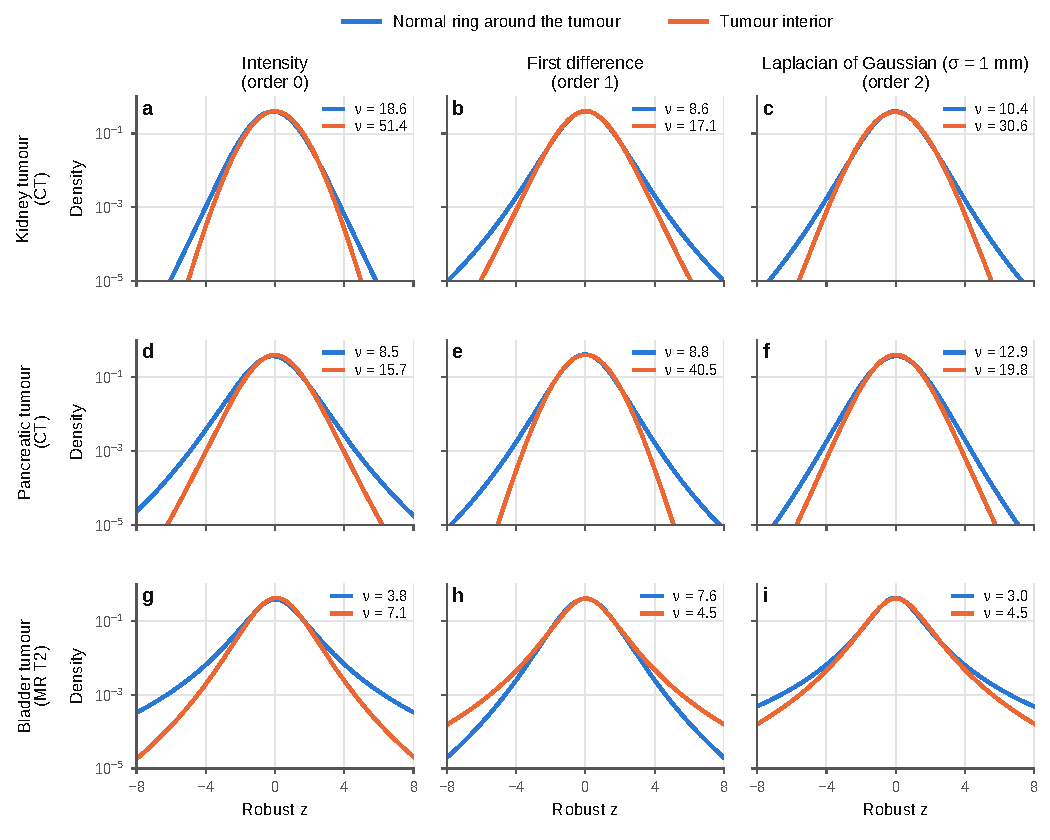
\includegraphics[width=\textwidth]{figs/stage2_tail_fits.pdf}}{\fbox{\parbox{0.9\linewidth}{\centering figs/stage2\_tail\_fits.pdf not found}}}
\caption{Student-$t$ fits of the tumor interior and the surrounding normal ring for one representative scan per site
(kidney and pancreas, CT; bladder, MR T2: the scan whose tumor and ring $\nu$ are closest to the site medians over the three
statistics), for the intensity (order 0), its first in-plane difference (order 1) and the Laplacian of Gaussian at
$\sigma=1$\,mm (order 2). Both regions are fitted at equal sample size on a 3\,mm grid and shown in robust $z$ units (median,
$1.4826\times$MAD). Lower $\nu$ means heavier tails.}
\label{fig:stage2_tail_fits}
\end{figure*}

\begin{figure*}[t]
\centering
\IfFileExists{figs/stage2_tail_nu.pdf}{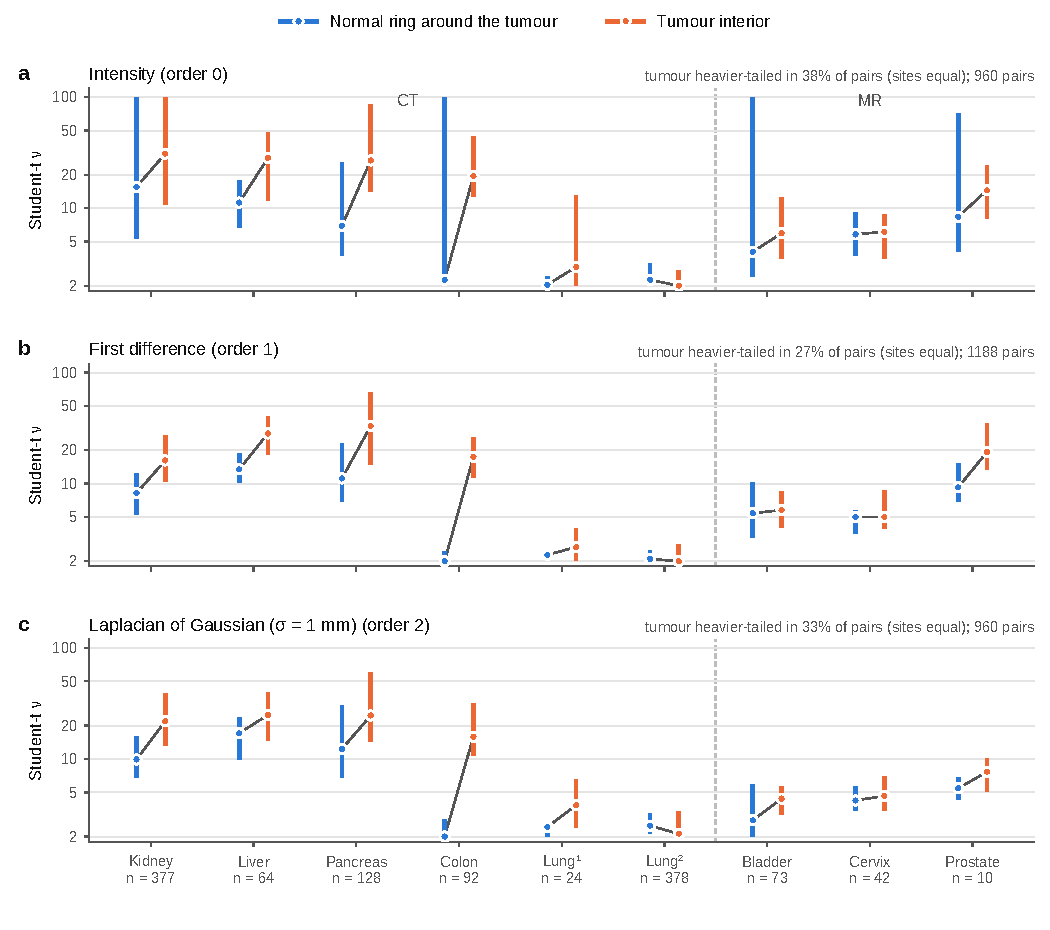
\includegraphics[width=\textwidth]{figs/stage2_tail_nu.pdf}}{\fbox{\parbox{0.9\linewidth}{\centering figs/stage2\_tail\_nu.pdf not found}}}
\caption{Student-$t$ $\nu$ of the tumor interior and the surrounding normal ring per collection (median and interquartile
range; medians connected) for (a) intensity, (b) first difference and (c) Laplacian of Gaussian. Pairs are from the same
scan, fitted at equal sample size ($\ge200$ voxels); $\nu$ is bounded to $[2,100]$. Lung$^1$: MSD lung; Lung$^2$: NSCLC. $n$:
pairs for the first difference (the other statistics need more clearance and have fewer pairs). Breast has no segmented host
organ.}
\label{fig:stage2_tail_nu}
\end{figure*}

\begin{figure*}[t]
\centering
\IfFileExists{figs/stage2_tail_scale.pdf}{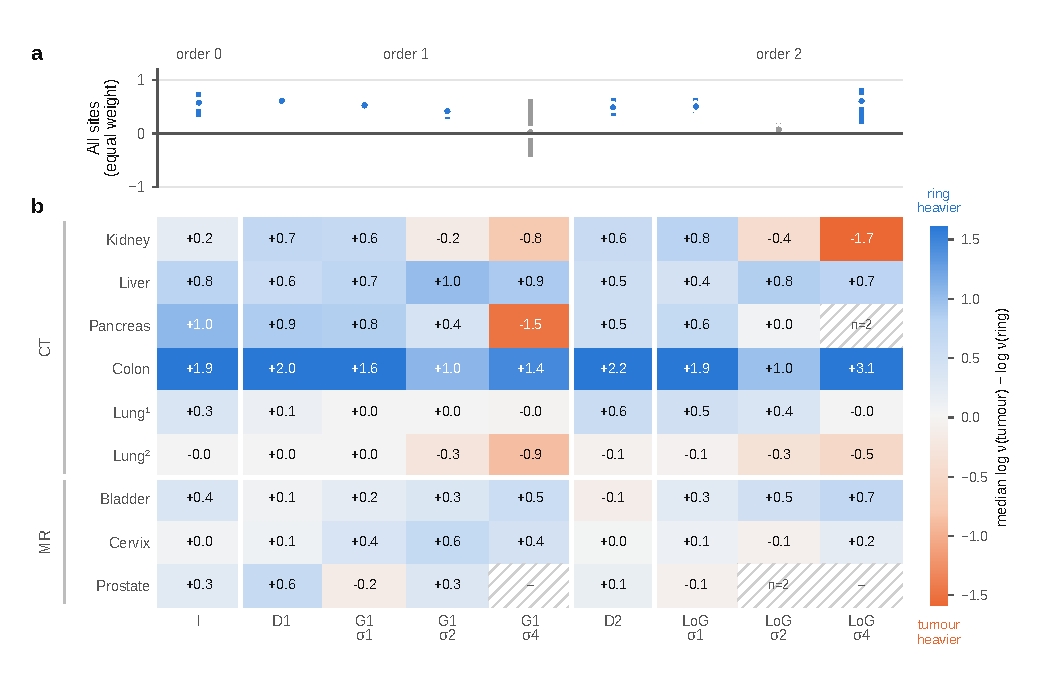
\includegraphics[width=\textwidth]{figs/stage2_tail_scale.pdf}}{\fbox{\parbox{0.9\linewidth}{\centering figs/stage2\_tail\_scale.pdf not found}}}
\caption{Paired difference of tail weight, $\log\nu_{\mathrm{tumor}}-\log\nu_{\mathrm{ring}}$, by statistic and scale. (a)~All
sites with equal weight: mean of the site medians with a stratified bootstrap 95\% interval (blue: ring heavier-tailed; grey:
interval includes 0). (b)~Median per collection; hatched: fewer than 5 pairs. I: intensity; D1, D2: first difference and
discrete Laplacian; G1, LoG: Gaussian derivative and Laplacian of Gaussian at $\sigma$ in mm.}
\label{fig:stage2_tail_scale}
\end{figure*}

\begin{figure*}[t]
\centering
\IfFileExists{figs/stage2_tail_reference.pdf}{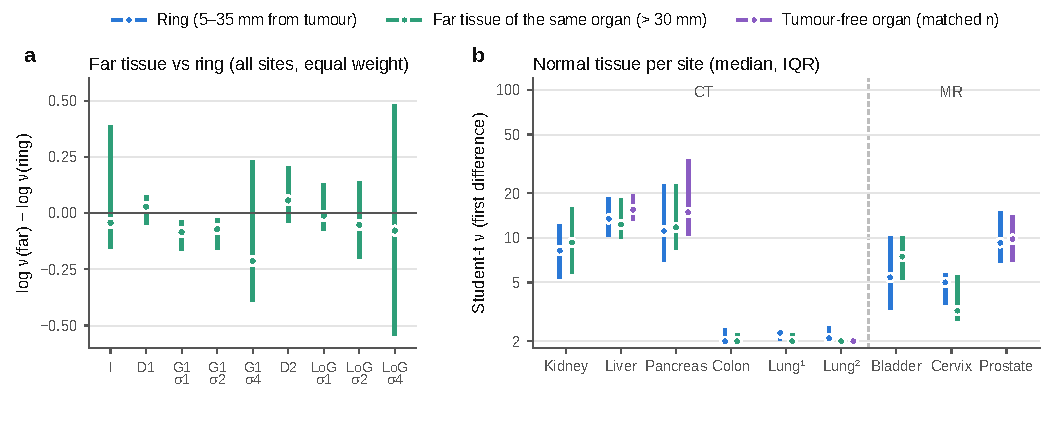
\includegraphics[width=\textwidth]{figs/stage2_tail_reference.pdf}}{\fbox{\parbox{0.9\linewidth}{\centering figs/stage2\_tail\_reference.pdf not found}}}
\caption{The ring as a normal reference. (a)~Paired difference $\log\nu_{\mathrm{far}}-\log\nu_{\mathrm{ring}}$ between far tissue
of the same organ ($>30$\,mm from every tumor) and the ring, all sites with equal weight (95\% interval). (b)~$\nu$ of the first
difference in the ring, far tissue and tumor-free organs of the same collection (median, interquartile range; tumor-free organs
fitted at the sample size closest to the rings'). Collections without far tissue or tumor-free scans show fewer groups.}
\label{fig:stage2_tail_reference}
\end{figure*}

\begin{figure*}[t]
\centering
\IfFileExists{figs/stage2_tail_structure.pdf}{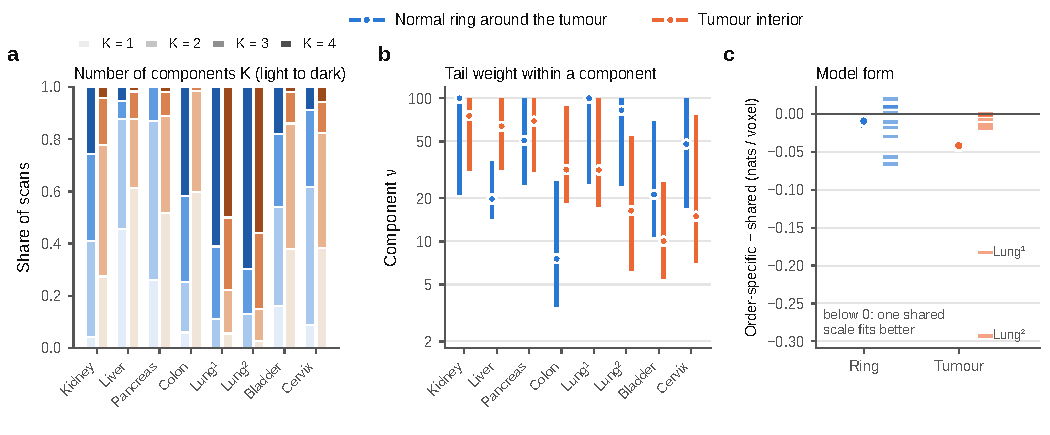
\includegraphics[width=\textwidth]{figs/stage2_tail_structure.pdf}}{\fbox{\parbox{0.9\linewidth}{\centering figs/stage2\_tail\_structure.pdf not found}}}
\caption{Substructure and model form on the joint features (intensity, two first differences, Laplacian of Gaussian at 1\,mm).
(a)~Number of Student-$t$ components chosen by the lower bound (1 to 4, light to dark), ring (left bar) and tumor (right bar).
(b)~$\nu$ of the components (weight $\ge0.05$, $\ge100$ voxels; median, interquartile range). (c)~Lower bound per voxel of
order-specific scales minus one shared scale, with the effect of cross-order correlation removed: all sites with equal weight
(dot, 95\% interval) and collection medians (dashes). Prostate is omitted for its few pairs.}
\label{fig:stage2_tail_structure}
\end{figure*}

\paragraph{Components.} No substructure annotations exist, so the number of components is inferred. $K_{\max}=4$ is the
number of tissue types a radiologist distinguishes in a solid tumor (enhancing solid tissue, necrosis, cystic or fluid
content, calcification or haemorrhage), and $\alpha_0=\tfrac14$; both are disclosed design values. Components are unlabelled
during inference; a name is attached afterwards from their appearance relative to the host's normal tissue and is reported as
a description, never used in a decision.

\paragraph{Outputs.} Trimmed voxels $\hat\xi_L\setminus\hat Z_L$ and recalled voxels $\hat Z_L\setminus\hat\xi_L$ are reported
with the host territories they lie in. Lesions of a cluster whose refined tumors meet are reported as merged. New candidates
(components of $\{p_v\ge\tfrac12\}$ meeting no anchor) are reported with their distance to the nearest anchor; they can be
benign findings, and no rule is applied to them before review. Recall comes from the image and the spatial prior only; the
agents' discarded proposals are never re-admitted.

\paragraph{Bayes factor.} $N_L=(\bigcup_{a\in L}a)\oplus r$ within the region, so that abnormal tissue elsewhere in a large
host does not count for the lesion, and it must contain normal tissue around the claim. Both models are refitted on $N_L$
with the same within-scan priors and \emph{matched flexibility}: the background-only model gets $K_{\max}$ extra free
background classes, and the tumor model adds $K_{\max}$ tumor classes placed by the spatial prior. Without the extra classes,
the model with more components always won. A ratio of lower bounds approximates the Bayes factor; it treats voxels as
independent, so only its sign is used, and it is also reported per voxel. The threshold $1$ is where both models are equally
supported. The stage-1 existence evidence is also recomputed on $\hat Z_L$ under each credible host, with the same tables and
$\alpha$, and reported next to the stage-1 outcome; it does not change decisions.

\paragraph{Estimation and validation.} Estimated on expert data: $\eta$, $r$, $(a_\omega,b_\omega)$ and the tail-weight
priors per cell (Table~\ref{tab:nu_prior}).
Design values: $K_{\max}$, $\alpha_0$, the basis knots, the $L_2$ penalty and the run settings (at most $300$ iterations).
Validation holds out one tumor site at a time (the two lung collections together) and refits on the others. It reports, per
site and organ class, voxel precision and recall, Dice, the over- and under-segmented fractions and the calibration of
$p_v$, against the chosen extent, $q^L_v$ thresholded at $\tfrac12$, the anchor alone and the union of outlines; recall beyond
the union of candidate extents by distance band; and the Bayes-factor flag rates for true anchors, false anchors in tumor
scans and anchors in tumor-free scans. All summaries weight sites equally. Stage~2 replaces the stage-1 extent only where it
improves the held-out Dice.

\paragraph{Evaluation of components.} Without substructure annotations, components are compared with radiological reads.
The TCGA-KIRC radiogenomic table (radiologists' reads distributed with the cohort; source citation to be added) records, per
patient, solid composition, necrosis, calcification, margin and growth pattern; $95$ of its patients have a segmented
baseline series in our cohort ($74$ CT, $21$ MR). The presence and volume fraction of each inferred component are compared
with these reads. Lesions are matched to reads by side and tumor count; patients whose tumors cannot be matched are left out
and counted. The reads are used for evaluation only, and no clinical or demographic variable of the table is used.


\section{Constants}
\label{app:constants}
Table~\ref{tab:constants} lists the constants of stage~1 and their sources; stage-2 design values are listed in
Appendix~\ref{sec:stage2_details}.

\begin{table*}[t]
\centering\footnotesize
\caption{Constants of stage~1 and their source: \emph{expert} (estimated on public expert
annotations, R2Seg and TotalSegmentator; held out where evaluated), \emph{KB} (knowledge base), \emph{design} (chosen a priori,
with the reason; sensitivity reported). No constant is estimated on TCGA or on stage.}
\label{tab:constants}
\setlength{\tabcolsep}{3pt}
\begin{tabular}{p{0.30\linewidth}p{0.20\linewidth}p{0.10\linewidth}p{0.36\linewidth}}
\hline
Constant & Value & Source & Note\\
\hline
Host weights & equal & design & $\mathcal{H}_C$ decides candidates only; roles attached after inference\\
Envelope, lesion distance $\tau$ & $10$\,mm, $10$\,mm & design & tumor displacement; fixed in mm (not slice spacing)\\
Mask confidence $\mu$ & $1$, $\tfrac12$, $0$ & design & feasible / anatomy violated / corrupt or impossible\\
Organ checks (volume, side, span, contact) & $2v_{\max}$, $0.5v_{\min}$, $10$\,mm, span$\pm$(var$+1$) & KB & lower $\mu$; never remove\\
Compatibility weights $\beta$ & fitted (choice model) & expert & testbed host cases incl.\ knowledge-base regions [to be refitted]\\
Ridge penalties & $\tfrac12\|\beta\|^2$; $0.01\|\theta\|^2$ & design & host choice model; extent prior\\
Host credible set & probability $\ge1-\alpha$ & design ($\alpha$) & smallest such set of candidates\\
Knowledge-base region (unsegmented) & own span$\pm$(var$+\tfrac12$) levels & KB & sided, in body; out of view if $<50\%$ of span in scan\\
Organs outside $\mathcal{H}_C$ as candidates & $\mu_o=1$, span in view $\ge50\%$ & design & never a knowledge-base region\\
Support levels $\ell$ & $2$ / $1$ / $0$ & design & ordinal: two agents $>$ one agent; each warning signal $-1$\\
Error level $\alpha$ & $0.05$ & design & significance level of the existence test; sensitivity $\{0.01,0.10\}$\\
Lobe opening, minimum & $3$\,mm ball, $0.5$\,ml & design & neck narrower than $\sim6$\,mm\\
Claim minimum, crumbs & $0.5$\,ml; $0.2$\,ml within $5$\,mm & design & as v6\\
Prompt mismatch, flatness & $<50\%$ in envelope; aspect $\le0.25$, coverage $\ge40\%$ & design & warning signals only\\
Organ-overlap tests & $0.6$ / $0.6$ / $0.8$; $0.8$ / $0.5$ & design & as v6 (D10)\\
Parsimony $\psi$ & piecewise on $\log(|\xi|/|a|)$ & expert & bins $<0.05,0.4,0.8,1.2,1.8,2.5,\infty$ [to be refitted with $\eta_f$]\\
Flag factors $\eta_f$ & $\le1$ & expert & fitted jointly with $\psi$ (held out by collection); no-example flags take the smallest\\
Extent evidence & not used & expert & did not improve extent choice on held-out expert data (ablation)\\
Normal reference & $2$\,mm margin, $200$ voxels in $50$\,mm & design & as G0\\
Sign thresholds (closed, open, patchy, elongated, deviation) & $1.42$, $5.27$, $1.047$, $0.363$, $1.5$ & expert & percentiles of expert data (frozen 12 Oct)\\
Tables (strata, smoothing) & $\ge30$; $\kappa=0.2$ & expert & $\kappa$ by held-out likelihood over $\{0,\dots,5\}$; $n/(n+10)$ for reported $\Lambda$ only\\
Common grid & $\sim5$\,mm through-plane & expert & thickening changes signs; small-lesion check\\
Decision & Table~\ref{tab:decision} & design & a conflict gives uncertain\\
Quality control & $f\ge0.25$, $0.5$; $8$\,mm; $76.6$\,HU, SNR $1.64$ & expert/design & noise percentiles of expert data\\
\hline
\end{tabular}
\end{table*}

\end{document}
